% psmc-rs manuscript. Build with `tectonic psmc-rs.tex` in this directory
% (manuscript/README.md). Every result quoted is a macro of numbers.tex,
% generated by make_numbers.py from the committed results; Tables 1, 2 and
% S1 are generated the same way.
\documentclass[11pt]{article}
\usepackage[a4paper,margin=2.5cm]{geometry}
\usepackage{amsmath}
\usepackage{fontspec}
\setmainfont{texgyretermes}[Extension=.otf,UprightFont=*-regular,BoldFont=*-bold,ItalicFont=*-italic,BoldItalicFont=*-bolditalic]
\usepackage{unicode-math}
\setmathfont{texgyretermes-math.otf}
\usepackage{graphicx}
\usepackage{booktabs}
\usepackage{xcolor}
\usepackage[round]{natbib}
\usepackage{microtype}
\usepackage{setspace}
\usepackage{caption}
\usepackage[hidelinks]{hyperref}
\usepackage{xurl}
\usepackage{lineno}
\usepackage{placeins}
\captionsetup{font=small,labelfont=bf,labelsep=period}
\graphicspath{{../experiment/runs/}}
\setlength{\bibsep}{2pt}
\setlength{\emergencystretch}{1.5em}
\renewcommand{\topfraction}{0.92}
\renewcommand{\bottomfraction}{0.8}
\renewcommand{\textfraction}{0.06}
\renewcommand{\floatpagefraction}{0.85}
\setcounter{topnumber}{2}
\setcounter{totalnumber}{3}
% Generated by manuscript/make_numbers.py from experiment/runs/*/tables; do not edit.

\newcommand{\EoneModels}{4}  % config.E1.models
\newcommand{\EoneReps}{10}  % config.E1.replicates
\newcommand{\EoneGenomes}{40}  % models x replicates
\newcommand{\EoneChroms}{10}  % config.E1.genome
\newcommand{\EoneChromMb}{50}  % config.E1.genome
\newcommand{\EoneGenomeMb}{500}  % config.E1.genome
\newcommand{\EoneRsCRmseMin}{\ensuremath{3.7\times10^{-6}}}  % E1_rs_vs_c min rmse
\newcommand{\EoneRsCRmseMax}{\ensuremath{2.0\times10^{-4}}}  % E1_rs_vs_c max rmse
\newcommand{\EoneRsCRmseMedian}{\ensuremath{2.5\times10^{-5}}}  % E1_rs_vs_c median rmse
\newcommand{\EoneRsCMaxAbs}{\ensuremath{6.6\times10^{-4}}}  % E1_rs_vs_c max abs in window
\newcommand{\EoneAnyMax}{\ensuremath{2.0}}  % E1_rs_vs_c max abs any interval
\newcommand{\EoneAnyModel}{expansion}  % E1_rs_vs_c worst any interval
\newcommand{\EoneAnyReplicate}{5}  % E1_rs_vs_c worst any interval
\newcommand{\EoneAnySecond}{\ensuremath{6.6\times10^{-4}}}  % E1_rs_vs_c second largest any interval
\newcommand{\EoneRunawayC}{\ensuremath{1.1\times10^{6}}}  % E1_curves worst replicate, C psmc's first lambda
\newcommand{\EoneRunawayCNe}{\ensuremath{2.5\times10^{9}}}  % E1_curves worst replicate, C psmc's Ne in the first interval
\newcommand{\EoneRunawayKy}{\ensuremath{4.8}}  % E1_curves worst replicate, end of the first free lambda (ky)
\newcommand{\EoneParamRelMax}{\ensuremath{5.5\times10^{-4}}}  % E1_rs_vs_c max |rel diff| theta, rho, t_max
\newcommand{\EoneLoglikeRelMax}{\ensuremath{3.5\times10^{-8}}}  % E1_rs_vs_c loglike_max_rel_diff (any iteration)
\newcommand{\EoneLoglikeLastRelMax}{\ensuremath{1.3\times10^{-8}}}  % E1_replicates loglike_common (the last iteration both report)
\newcommand{\EoneLoglikeFirstRelMax}{\ensuremath{7.0\times10^{-13}}}  % E1_rs_vs_c loglike_iteration0_rel_diff
\newcommand{\EoneConstantTruthC}{\ensuremath{0.048}}  % E1_table1 rmse_truth_c_mean
\newcommand{\EoneConstantTruthRs}{\ensuremath{0.048}}  % E1_table1 rmse_truth_rs_mean
\newcommand{\EoneBottleneckTruthC}{\ensuremath{0.291}}  % E1_table1 rmse_truth_c_mean
\newcommand{\EoneBottleneckTruthRs}{\ensuremath{0.291}}  % E1_table1 rmse_truth_rs_mean
\newcommand{\EoneExpansionTruthC}{\ensuremath{0.240}}  % E1_table1 rmse_truth_c_mean
\newcommand{\EoneExpansionTruthRs}{\ensuremath{0.240}}  % E1_table1 rmse_truth_rs_mean
\newcommand{\EoneZigzagTruthC}{\ensuremath{0.138}}  % E1_table1 rmse_truth_c_mean
\newcommand{\EoneZigzagTruthRs}{\ensuremath{0.138}}  % E1_table1 rmse_truth_rs_mean
\newcommand{\EoneMonotoneRuns}{80}  % E6_S1_summary replicates_monotone
\newcommand{\EoneRuns}{80}  % E6_S1_summary replicates
\newcommand{\EtwoRsCRmseMin}{\ensuremath{9.7\times10^{-6}}}  % E2_rs_vs_c
\newcommand{\EtwoRsCRmseMax}{\ensuremath{2.8\times10^{-4}}}  % E2_rs_vs_c
\newcommand{\EtwoRsCMaxAbs}{\ensuremath{4.5\times10^{-4}}}  % E2_rs_vs_c
\newcommand{\EtwoHumanRmse}{\ensuremath{9.7\times10^{-6}}}  % E2_rs_vs_c NA12878
\newcommand{\EtwoParamRelMax}{\ensuremath{1.0\times10^{-3}}}  % E2_fit_summary theta, rho, t_max
\newcommand{\EtwoLoglikeRelMax}{\ensuremath{2.3\times10^{-7}}}  % E2_fit_summary loglike_common
\newcommand{\EtwoLoglikeFirstRelMax}{\ensuremath{6.9\times10^{-14}}}  % E2_rs_vs_c loglike_iteration0_rel_diff
\newcommand{\EtwoHumanSequences}{22}  % E2_fit_summary NA12878 sequences
\newcommand{\EtwoTurtleSeqMin}{34}  % E2_fit_summary turtle sequences
\newcommand{\EtwoTurtleSeqMax}{1,220}  % E2_fit_summary turtle sequences
\newcommand{\EtwoHumanTrunks}{59}  % E2_bootstrap NA12878 trunks
\newcommand{\EtwoBootReps}{100}  % E2_bootstrap replicates
\newcommand{\EtwoBootIdentical}{all}  % E2_bootstrap main_identical_to_fit
\newcommand{\EtwoBootThreads}{50}  % E2_bootstrap threads
\newcommand{\EtwoBandWidthMin}{\ensuremath{0.07}}  % E2_bootstrap band_width_log10_median
\newcommand{\EtwoBandWidthMax}{\ensuremath{0.15}}  % E2_bootstrap band_width_log10_median
\newcommand{\EtwoPeakMin}{\ensuremath{1.4}}  % E2_split_patterns default recent_max_vs_plateau
\newcommand{\EtwoPeakMax}{\ensuremath{4.6}}  % E2_split_patterns default recent_max_vs_plateau
\newcommand{\EtwoPeaksDefault}{3}  % E2_split_patterns default recent_peak
\newcommand{\EtwoPeaksSplit}{0}  % E2_split_patterns split recent_peak
\newcommand{\EtwoSplitFits}{6}  % E2_split_patterns split rows
\newcommand{\EtwoSplitGainMin}{\ensuremath{49}}  % E2_split_patterns loglike_gain_vs_default
\newcommand{\EtwoSplitGainMax}{\ensuremath{586}}  % E2_split_patterns loglike_gain_vs_default
\newcommand{\EtwoSplitOlderMax}{\ensuremath{1.5\times10^{-2}}}  % E2_split_curves: split vs default after the recent intervals, same times
\newcommand{\EtwoSplitThetaMax}{6.8\%}  % E2_split_patterns theta of split vs default
\newcommand{\EtwoBootPeakEmy}{56}  % E2_bootstrap_replicates recent_peak, E. subglobosa
\newcommand{\EtwoBootPeakHyd}{100}  % E2_bootstrap_replicates recent_peak, H. tectifera
\newcommand{\EtwoBootPeakPel}{100}  % E2_bootstrap_replicates recent_peak, P. castaneus
\newcommand{\EtwoTurtles}{3}  % E2_fit_summary turtle genomes
\newcommand{\EthreeRepeats}{5}  % config.E3.repeats
\newcommand{\EthreeBigMb}{3,000}  % config.E3.genome_sizes_mb
\newcommand{\EthreeBigChroms}{30}  % E3_table2 chromosomes
\newcommand{\EthreeCWall}{4,446}  % E3_table2 c 1 thread
\newcommand{\EthreeCMin}{\ensuremath{74}}  % E3_table2 c 1 thread (min)
\newcommand{\EthreeRsOneWall}{519}  % E3_table2 rs02 1 thread
\newcommand{\EthreeRsZeroWall}{6,193}  % E3_table2 rs01 1 thread
\newcommand{\EthreeSpeedOne}{\ensuremath{8.6}}  % E3_table2 rs02 1 speedup
\newcommand{\EthreeRsWallOne}{\ensuremath{519}}  % E3_table2 rs02 1 wall
\newcommand{\EthreeSpeedEight}{\ensuremath{63}}  % E3_table2 rs02 8 speedup
\newcommand{\EthreeRsWallEight}{\ensuremath{70.6}}  % E3_table2 rs02 8 wall
\newcommand{\EthreeSpeedSixteen}{\ensuremath{123}}  % E3_table2 rs02 16 speedup
\newcommand{\EthreeRsWallSixteen}{\ensuremath{36.0}}  % E3_table2 rs02 16 wall
\newcommand{\EthreeSpeedThirty}{\ensuremath{243}}  % E3_table2 rs02 30 speedup
\newcommand{\EthreeRsWallThirty}{\ensuremath{18.3}}  % E3_table2 rs02 30 wall
\newcommand{\EthreeRsZeroSpeedThirty}{\ensuremath{14}}  % E3_table2 rs01 30 speedup
\newcommand{\EthreeRsZeroRel}{\ensuremath{0.72}}  % E3_table2 rs01 1 speedup
\newcommand{\EthreeCMem}{1,062}  % E3_table2 c peak MB
\newcommand{\EthreeRsMemOne}{\ensuremath{36}}  % E3_table2 rs02 1 peak MB
\newcommand{\EthreeRsMemThirty}{\ensuremath{148}}  % E3_table2 rs02 30 peak MB
\newcommand{\EthreeRsZeroMemThirty}{14,959}  % E3_table2 rs01 30 peak MB
\newcommand{\EthreeRsZeroMemOne}{2,511}  % E3_table2 rs01 1 peak MB
\newcommand{\EthreeSpeedOneMin}{\ensuremath{8.5}}  % E3_table2 rs02 1 thread speedup, every size
\newcommand{\EthreeSpeedOneMax}{\ensuremath{8.8}}  % E3_table2 rs02 1 thread speedup, every size
\newcommand{\EthreeChromWall}{\ensuremath{17.3}}  % E3_table2 rs02 one 100 Mb chromosome, 1 thread
\newcommand{\EthreeChromWallMin}{\ensuremath{17.24}}  % E3_table2 rs02 100 Mb, any threads
\newcommand{\EthreeChromWallMax}{\ensuremath{17.25}}  % E3_table2 rs02 100 Mb, any threads
\newcommand{\EthreeRoundMin}{\ensuremath{17.2}}  % E3_table2 rs02 wall / ceil(chromosomes / threads)
\newcommand{\EthreeRoundMax}{\ensuremath{18.3}}  % E3_table2 rs02 wall / ceil(chromosomes / threads)
\newcommand{\EthreeEffMin}{\ensuremath{0.90}}  % E3_thread_scaling efficiency
\newcommand{\EthreeEffMax}{\ensuremath{0.99}}  % E3_thread_scaling efficiency
\newcommand{\EthreeEffCap}{\ensuremath{0.94}}  % whole chromosomes per thread: min over t of n / (t ceil(n / t))
\newcommand{\EthreeRuns}{155}  % E3_runs rows
\newcommand{\EthreeCleanRuns}{155}  % E3_runs clean
\newcommand{\EthreeNodes}{5}  % E3_runs hostname
\newcommand{\EthreeSpreadMaxMost}{3.5\%}  % E3_table2 (max-min)/median, second largest
\newcommand{\EthreeDetRsIdentical}{75}  % E3_determinism rs02
\newcommand{\EthreeDetRsTotal}{75}  % E3_determinism rs02
\newcommand{\EthreeDetCIdentical}{20}  % E3_determinism c
\newcommand{\EthreeDetCTotal}{20}  % E3_determinism c
\newcommand{\EthreeDetRsZeroIdentical}{30}  % E3_determinism rs01
\newcommand{\EthreeDetRsZeroTotal}{60}  % E3_determinism rs01
\newcommand{\EthreeRsZeroDiffMax}{\ensuremath{2.5\times10^{-5}}}  % E3_determinism rs01 max_rel_diff_params
\newcommand{\EthreeCpu}{AMD EPYC 7702}  % E3_environment machine.cpu
\newcommand{\EthreeCores}{128}  % E3_environment machine.cpu_count
\newcommand{\EfourDispThirtyFqTheta}{34.9\%}  % E4_routes dispersed30 fq2psmcfa -theta_rel (median)
\newcommand{\EfourDispThirtyFqRmse}{\ensuremath{0.36}}  % E4_routes dispersed30 fq2psmcfa rmse vs complete
\newcommand{\EfourDispThirtyAutoTheta}{1.8\%}  % E4_routes dispersed30 mask_auto -theta_rel (median)
\newcommand{\EfourDispThirtyAutoRmse}{\ensuremath{0.07}}  % E4_routes dispersed30 mask_auto rmse vs complete
\newcommand{\EfourDispThirtyNomaskTheta}{35.5\%}  % E4_routes dispersed30 nomask -theta_rel (median)
\newcommand{\EfourDispThirtyNomaskRmse}{\ensuremath{0.37}}  % E4_routes dispersed30 nomask rmse vs complete
\newcommand{\EfourDispThirtyMhsTheta}{31.9\%}  % E4_routes dispersed30 multihetsep -theta_rel (median)
\newcommand{\EfourDispThirtyMhsRmse}{\ensuremath{0.32}}  % E4_routes dispersed30 multihetsep rmse vs complete
\newcommand{\EfourDispTenFqTheta}{11.9\%}  % E4_routes dispersed10 fq2psmcfa -theta_rel (median)
\newcommand{\EfourDispTenFqRmse}{\ensuremath{0.19}}  % E4_routes dispersed10 fq2psmcfa rmse vs complete
\newcommand{\EfourDispTenAutoTheta}{0.7\%}  % E4_routes dispersed10 mask_auto -theta_rel (median)
\newcommand{\EfourDispTenAutoRmse}{\ensuremath{0.04}}  % E4_routes dispersed10 mask_auto rmse vs complete
\newcommand{\EfourDispTenNomaskTheta}{12.1\%}  % E4_routes dispersed10 nomask -theta_rel (median)
\newcommand{\EfourDispTenNomaskRmse}{\ensuremath{0.20}}  % E4_routes dispersed10 nomask rmse vs complete
\newcommand{\EfourDispTenMhsTheta}{17.0\%}  % E4_routes dispersed10 multihetsep -theta_rel (median)
\newcommand{\EfourDispTenMhsRmse}{\ensuremath{0.24}}  % E4_routes dispersed10 multihetsep rmse vs complete
\newcommand{\EfourClusThirtyFqTheta}{2.3\%}  % E4_routes clustered30 fq2psmcfa -theta_rel (median)
\newcommand{\EfourClusThirtyFqRmse}{\ensuremath{0.08}}  % E4_routes clustered30 fq2psmcfa rmse vs complete
\newcommand{\EfourClusThirtyAutoTheta}{2.2\%}  % E4_routes clustered30 mask_auto -theta_rel (median)
\newcommand{\EfourClusThirtyAutoRmse}{\ensuremath{0.08}}  % E4_routes clustered30 mask_auto rmse vs complete
\newcommand{\EfourClusThirtyNomaskTheta}{56.8\%}  % E4_routes clustered30 nomask -theta_rel (median)
\newcommand{\EfourClusThirtyNomaskRmse}{\ensuremath{0.50}}  % E4_routes clustered30 nomask rmse vs complete
\newcommand{\EfourClusThirtyMhsTheta}{9.1\%}  % E4_routes clustered30 multihetsep -theta_rel (median)
\newcommand{\EfourClusThirtyMhsRmse}{\ensuremath{0.18}}  % E4_routes clustered30 multihetsep rmse vs complete
\newcommand{\EfourReps}{5}  % config.E4.replicates
\newcommand{\EfourDispTenPartly}{48\%}  % E4_summary dispersed10 mask_auto
\newcommand{\EfourDispThirtyPartly}{92\%}  % E4_summary dispersed30 mask_auto
\newcommand{\EfourClusRunKb}{\ensuremath{20}}  % config.E4.masks mean uncallable run
\newcommand{\EfourDispRunBp}{\ensuremath{20}}  % config.E4.masks mean uncallable run
\newcommand{\EfourGenomeMb}{500}  % config.E4.genome
\newcommand{\EfiveFits}{50}  % E5_summary fits
\newcommand{\EfiveDatasets}{10}  % E5_summary datasets
\newcommand{\EfiveReps}{50}  % E5_summary replicates_per_dataset
\newcommand{\EfiveGenomeMb}{300}  % config.E5.genome
\newcommand{\EfiveChroms}{6}  % config.E5.genome
\newcommand{\EfiveFiftySd}{\ensuremath{0.84}}  % E5_summary sd_ratio_median
\newcommand{\EfiveFiftySdLo}{\ensuremath{0.78}}  % E5_summary sd_ratio_median_ci_lo
\newcommand{\EfiveFiftySdHi}{\ensuremath{0.92}}  % E5_summary sd_ratio_median_ci_hi
\newcommand{\EfiveFiftyCov}{37\%}  % E5_summary coverage_mean
\newcommand{\EfiveFiftyCovLo}{31\%}  % E5_summary coverage_mean_ci_lo
\newcommand{\EfiveFiftyCovHi}{43\%}  % E5_summary coverage_mean_ci_hi
\newcommand{\EfiveFiftyCovProj}{44\%}  % E5_summary coverage_projected_mean
\newcommand{\EfiveFiftyCovMean}{83\%}  % E5_summary coverage_of_fit_mean_mean
\newcommand{\EfiveFiftyTrunks}{6}  % E5_summary trunks
\newcommand{\EfiveFiveSd}{\ensuremath{0.93}}  % E5_summary sd_ratio_median
\newcommand{\EfiveFiveSdLo}{\ensuremath{0.91}}  % E5_summary sd_ratio_median_ci_lo
\newcommand{\EfiveFiveSdHi}{\ensuremath{0.97}}  % E5_summary sd_ratio_median_ci_hi
\newcommand{\EfiveFiveCov}{43\%}  % E5_summary coverage_mean
\newcommand{\EfiveFiveCovLo}{38\%}  % E5_summary coverage_mean_ci_lo
\newcommand{\EfiveFiveCovHi}{48\%}  % E5_summary coverage_mean_ci_hi
\newcommand{\EfiveFiveCovProj}{50\%}  % E5_summary coverage_projected_mean
\newcommand{\EfiveFiveCovMean}{92\%}  % E5_summary coverage_of_fit_mean_mean
\newcommand{\EfiveFiveTrunks}{60}  % E5_summary trunks
\newcommand{\EfiveBias}{\ensuremath{0.061}}  % E5_summary abs_bias_log10_median
\newcommand{\EfiveSdTrue}{\ensuremath{0.028}}  % E5_summary sd_true_log10_median
\newcommand{\EsixVcfIdentical}{all}  % E6_S2_fits vcf identical
\newcommand{\EsixMhsMaxAbs}{\ensuremath{0.024}}  % E6_S2_fits multihetsep max abs
\newcommand{\EsixMhsDiffering}{0}  % E6_S2_bins multihetsep bins_differing
\newcommand{\EsixMhsTailMin}{116}  % E6_S2_bins multihetsep bins_missing_at_end (whole genome)
\newcommand{\EsixMhsTailMax}{1,430}  % E6_S2_bins multihetsep bins_missing_at_end (whole genome)
\newcommand{\EsixDecodeR}{\ensuremath{0.91}}  % E6_S3_summary pearson_log10_mean
\newcommand{\EsixDecodeCov}{95.6\%}  % E6_S3_summary coverage95_states
\newcommand{\EsixDecodeBins}{5,000,000}  % E6_S3_summary n_bins
\newcommand{\EsixTrueDecileMin}{90.1\%}  % E6_S3_calibration by true TMRCA
\newcommand{\EsixTrueDecileMax}{98.3\%}  % E6_S3_calibration by true TMRCA
\newcommand{\EsixPostDecileMin}{94.9\%}  % E6_S3_calibration by posterior mean
\newcommand{\EsixPostDecileMax}{96.9\%}  % E6_S3_calibration by posterior mean
\newcommand{\EsixYoungBias}{\ensuremath{0.19}}  % E6_S3_calibration true decile 1 bias
\newcommand{\EsixOldBias}{\ensuremath{0.13}}  % E6_S3_calibration true decile 10 -bias
\newcommand{\EsixSaturated}{2}  % E6_S5_qc BIN_SATURATION
\newcommand{\EsixSatShareLo}{11\%}  % E6_S5_qc multi_het_share
\newcommand{\EsixSatShareHi}{12\%}  % E6_S5_qc multi_het_share
\newcommand{\EsixSatBinLo}{40}  % E6_S5_qc max_bin_size_below_target
\newcommand{\EsixSatBinHi}{43}  % E6_S5_qc max_bin_size_below_target
\newcommand{\EsixShortSeq}{3}  % E6_S5_qc SHORT_SEQUENCES
\newcommand{\EsevenGenomes}{2,504}  % E7_samples rows
\newcommand{\EsevenPops}{26}  % E7_samples populations
\newcommand{\EsevenSups}{5}  % E7_samples superpopulations
\newcommand{\EsevenDefault}{52}  % E7_samples default
\newcommand{\EsevenPerPopMin}{61}  % E7_samples per population
\newcommand{\EsevenPerPopMax}{113}  % E7_samples per population
\newcommand{\EsevenDepth}{\ensuremath{36.2}}  % E7_inputs raw_depth median
\newcommand{\EsevenCallableGb}{\ensuremath{2.16}}  % E7_inputs callable_bases median
\newcommand{\EsevenPartly}{27\%}  % E7_inputs partly_callable_bin_fraction
\newcommand{\EsevenHetAfr}{\ensuremath{1.01}}  % E7_inputs het_per_callable_kb AFR
\newcommand{\EsevenHetEas}{\ensuremath{0.71}}  % E7_inputs het_per_callable_kb EAS
\newcommand{\EsevenMissingShare}{7.6\%}  % E7_route_shift missing share
\newcommand{\EsevenThetaShift}{8.4\%}  % E7_route_shift theta_rel mean
\newcommand{\EsevenThetaShiftLo}{7.9\%}  % E7_route_shift theta_rel min
\newcommand{\EsevenThetaShiftHi}{8.8\%}  % E7_route_shift theta_rel max
\newcommand{\EsevenNeShift}{\ensuremath{0.041}}  % E7_curves rs-vcf vs rs-psmcfa, mean log10 over the window at the same times
\newcommand{\EsevenRsCRmseMin}{\ensuremath{5.7\times10^{-6}}}  % E7_rs_vs_c
\newcommand{\EsevenRsCRmseMax}{\ensuremath{2.1\times10^{-5}}}  % E7_rs_vs_c
\newcommand{\EsevenRsCMaxAbs}{\ensuremath{5.8\times10^{-5}}}  % E7_rs_vs_c
\newcommand{\EsevenGiabPrecision}{\ensuremath{0.9992}}  % E7_giab precision
\newcommand{\EsevenGiabRecall}{\ensuremath{0.9966}}  % E7_giab recall
\newcommand{\EsevenGiabTruth}{1,564,410}  % E7_giab truth_het_snvs
\newcommand{\EsevenGiabMb}{2,109}  % E7_giab eval_bases (Mb)
\newcommand{\EsevenRsCoreHours}{502}  % E7_throughput rs-psmcfa core_hours
\newcommand{\EsevenRsFitMin}{12.1}  % E7_throughput rs-psmcfa wall median (min)
\newcommand{\EsevenCFitMin}{104.3}  % E7_throughput c wall median (min)
\newcommand{\EsevenCCoreHoursAll}{4,400}  % E7_throughput c wall median x genomes (estimate)
\newcommand{\EsevenSpeed}{\ensuremath{8.6}}  % E7_throughput c / rs-psmcfa wall median
\newcommand{\EsevenBootIdentical}{all}  % E7_bootstrap main_identical_to_fit
\newcommand{\EsevenBootReps}{100}  % E7_bootstrap replicates
\newcommand{\EsevenBootThreads}{32}  % E7_bootstrap threads
\newcommand{\EsevenBootMin}{37.5}  % E7_bootstrap wall median (min)
\newcommand{\EsevenSplitRmse}{\ensuremath{0.056}}  % E7_split rmse median
\newcommand{\EsevenSplitN}{26}  % E7_split rows
\newcommand{\EsevenMu}{\ensuremath{1.25\times10^{-8}}}  % config.E7.scaling
\newcommand{\EsevenG}{29}  % config.E7.scaling
\newcommand{\EsevenThetaExpected}{8.2\%}  % 1 / (1 - missing share) - 1
\newcommand{\EsevenRsCParamRelMax}{\ensuremath{5.4\times10^{-5}}}  % E7_rs_vs_c theta, rho, t_max
\newcommand{\EsevenRsCLoglikeFirst}{\ensuremath{1.1\times10^{-13}}}  % E7_rs_vs_c loglike_iteration0_rel_diff
\newcommand{\RealGenomes}{55}  % E2_rs_vs_c and E7_rs_vs_c samples (NA12878 in both)
\newcommand{\EsevenGiabCalled}{1,560,297}  % E7_giab called_het_snvs
\newcommand{\EsevenGiabFp}{1,174}  % E7_giab fp
\newcommand{\EsevenGiabFn}{5,287}  % E7_giab fn
\newcommand{\EsevenGiabFnIndel}{3,472}  % E7_giab fn_het_indel
\newcommand{\EsevenGiabFnNonpass}{1,402}  % E7_giab fn_nonpass
\newcommand{\EsevenRsMem}{\ensuremath{105}}  % E7_throughput rs-psmcfa peak MB
\newcommand{\EsevenCMemFit}{2,597}  % E7_throughput c peak MB
\newcommand{\EsevenVcfFitMin}{11.7}  % E7_throughput rs-vcf wall median (min)
\newcommand{\EsevenBootCoreHours}{59}  % E7_throughput boot-rs core_hours
\newcommand{\EsevenCCoreHours}{91}  % E7_throughput c core_hours
\newcommand{\EsevenBootSamples}{3}  % E7_bootstrap rows
\newcommand{\EsevenBootFiles}{103}  % E2/bootstrap and E7/boot NA12878 files
\newcommand{\EsevenBootFilesIdentical}{103}  % E2/bootstrap and E7/boot NA12878 files byte-identical
\newcommand{\EsevenBoundDefault}{0}  % E7_curves rs-psmcfa first window at 1e4
\newcommand{\EsevenSplitBound}{3}  % E7_curves rs-split first window at 1e4
\newcommand{\EsevenSplitRmseMax}{\ensuremath{0.78}}  % E7_split rmse max
\newcommand{\EsevenNonAfrMinNeLo}{1,961}  % E7_pop_bands non-AFR superpopulation minima
\newcommand{\EsevenNonAfrMinNeHi}{2,902}  % E7_pop_bands non-AFR superpopulation minima
\newcommand{\EsevenNonAfrMinKyLo}{\ensuremath{43}}  % E7_pop_bands non-AFR minima (ky)
\newcommand{\EsevenNonAfrMinKyHi}{\ensuremath{52}}  % E7_pop_bands non-AFR minima (ky)
\newcommand{\EsevenAfrMinNe}{9,422}  % E7_pop_bands AFR minimum
\newcommand{\EsevenAfrMinKy}{\ensuremath{68}}  % E7_pop_bands AFR minimum (ky)
\newcommand{\EsevenHumpNeLo}{28,969}  % E7_pop_bands local maxima 100 ky-2 My
\newcommand{\EsevenHumpNeHi}{30,396}  % E7_pop_bands local maxima 100 ky-2 My
\newcommand{\EsevenHumpKyLo}{\ensuremath{294}}  % E7_pop_bands local maxima (ky)
\newcommand{\EsevenHumpKyHi}{\ensuremath{330}}  % E7_pop_bands local maxima (ky)
\newcommand{\EsevenConvergeKy}{\ensuremath{247}}  % E7_pop_bands: superpopulation medians within 20% from here to the window's end
\newcommand{\EsevenWindowHiMy}{\ensuremath{4.6}}  % E7_pop_bands all window_hi_years (My)
\newcommand{\EsevenPopCutKy}{\ensuremath{150}}  % split of recent and older times for the populations' spread
\newcommand{\EsevenPopSpreadRecentLo}{\ensuremath{0.24}}  % E7_pop_bands populations of a superpopulation, max log10 spread < 150 ky (lowest)
\newcommand{\EsevenPopSpreadRecentHi}{\ensuremath{0.99}}  % E7_pop_bands populations of a superpopulation, max log10 spread < 150 ky (highest)
\newcommand{\EsevenPopSpreadOldMax}{\ensuremath{0.11}}  % E7_pop_bands populations of a superpopulation, max log10 spread >= 150 ky
\newcommand{\EsevenRecords}{123,574,606}  % MANIFEST chromosomes records
\newcommand{\EsevenNonpass}{11,256,876}  % MANIFEST chromosomes nonpass
\newcommand{\EsevenVcfTb}{\ensuremath{1.68}}  % MANIFEST chromosomes read bytes (TB)
\newcommand{\EsevenPilotChrom}{21}  % MANIFEST pilots
\newcommand{\EsevenPilotSamples}{3}  % MANIFEST pilots samples
\newcommand{\DiagCurve}{\ensuremath{7.7\times10^{-5}}}  % README.md Testing and C equivalence: DiagCurve
\newcommand{\DiagHookeJeeves}{\ensuremath{7.5\times10^{-5}}}  % README.md Testing and C equivalence: DiagHookeJeeves
\newcommand{\DiagLastBin}{\ensuremath{6.4\times10^{-6}}}  % README.md Testing and C equivalence: DiagLastBin
\newcommand{\DiagPrecision}{\ensuremath{5.0\times10^{-7}}}  % README.md Testing and C equivalence: DiagPrecision
\newcommand{\DiagChroms}{4}  % README.md Testing and C equivalence
\newcommand{\DiagChromMb}{25}  % README.md Testing and C equivalence
\newcommand{\XpGenomes}{40}  % crossplatform inputs_E1_genomes rows
\newcommand{\XpGenomesIdentical}{40}  % crossplatform inputs identical
\newcommand{\XpRsFits}{41}  % crossplatform rs fits
\newcommand{\XpRsBytesIdentical}{0}  % crossplatform rs JSON byte-identical
\newcommand{\XpCBytesIdentical}{0}  % crossplatform C .psmc byte-identical
\newcommand{\XpRsRmseMax}{\ensuremath{1.0\times10^{-6}}}  % crossplatform rs RMSE window max (E1)
\newcommand{\XpRsRmseMedian}{\ensuremath{1.2\times10^{-7}}}  % crossplatform rs RMSE window median (E1)
\newcommand{\XpRsParamMax}{\ensuremath{9.6\times10^{-6}}}  % crossplatform rs largest relative parameter difference (E1)
\newcommand{\XpCRmseMedian}{\ensuremath{8.5\times10^{-6}}}  % crossplatform C RMSE window median
\newcommand{\XpCRmseMax}{\ensuremath{2.4\times10^{-5}}}  % crossplatform C RMSE window max
\newcommand{\XpRatioCMedian}{\ensuremath{80}}  % side_by_side ratio C cross-build / rs cross-platform, median
\newcommand{\XpRatioCMin}{\ensuremath{7.2}}  % side_by_side ratio C cross-build / rs cross-platform, min
\newcommand{\XpRatioRsCMedian}{\ensuremath{196}}  % side_by_side ratio rs-vs-C / rs cross-platform, median
\newcommand{\XpRatioRsCMin}{\ensuremath{45}}  % side_by_side ratio rs-vs-C / rs cross-platform, min
\newcommand{\XpIterZero}{40}  % crossplatform rs iteration-0 log-likelihood identical
\newcommand{\XpTierB}{24}  % crossplatform rs E1 tier B
\newcommand{\XpTierC}{11}  % crossplatform rs E1 tier C
\newcommand{\XpTierFail}{5}  % crossplatform rs E1 tier fail
\newcommand{\XpCTierFail}{40}  % crossplatform C tier fail
\newcommand{\XpNaRmse}{\ensuremath{9.1\times10^{-8}}}  % crossplatform NA12878 RMSE window
\newcommand{\XpNaTier}{B}  % crossplatform NA12878 tier
\newcommand{\EoneModelsW}{four}  % config.E1.models (in words)
\newcommand{\EoneAnyReplicateW}{five}  % E1_rs_vs_c worst any interval (in words)
\newcommand{\EtwoPeaksDefaultW}{three}  % E2_split_patterns default recent_peak (in words)
\newcommand{\EtwoPeaksSplitW}{zero}  % E2_split_patterns split recent_peak (in words)
\newcommand{\EtwoSplitFitsW}{six}  % E2_split_patterns split rows (in words)
\newcommand{\EtwoTurtlesW}{three}  % E2_fit_summary turtle genomes (in words)
\newcommand{\EthreeRepeatsW}{five}  % config.E3.repeats (in words)
\newcommand{\EthreeNodesW}{five}  % E3_runs hostname (in words)
\newcommand{\EfourRepsW}{five}  % config.E4.replicates (in words)
\newcommand{\EfiveChromsW}{six}  % config.E5.genome (in words)
\newcommand{\EfiveFiftyTrunksW}{six}  % E5_summary trunks (in words)
\newcommand{\EsixMhsDifferingW}{zero}  % E6_S2_bins multihetsep bins_differing (in words)
\newcommand{\EsixSaturatedW}{two}  % E6_S5_qc BIN_SATURATION (in words)
\newcommand{\EsixShortSeqW}{three}  % E6_S5_qc SHORT_SEQUENCES (in words)
\newcommand{\EsevenSupsW}{five}  % E7_samples superpopulations (in words)
\newcommand{\EsevenBootSamplesW}{three}  % E7_bootstrap rows (in words)
\newcommand{\EsevenBoundDefaultW}{zero}  % E7_curves rs-psmcfa first window at 1e4 (in words)
\newcommand{\EsevenSplitBoundW}{three}  % E7_curves rs-split first window at 1e4 (in words)
\newcommand{\EsevenPilotSamplesW}{three}  % MANIFEST pilots samples (in words)
\newcommand{\DiagChromsW}{four}  % README.md Testing and C equivalence (in words)
\newcommand{\XpRsBytesIdenticalW}{zero}  % crossplatform rs JSON byte-identical (in words)
\newcommand{\XpCBytesIdenticalW}{zero}  % crossplatform C .psmc byte-identical (in words)
\newcommand{\XpTierFailW}{five}  % crossplatform rs E1 tier fail (in words)

\newcommand{\psmcrs}{psmc-rs}
\newcommand{\Ne}{\ensuremath{N_\mathrm{e}}}
\newcommand{\opt}[1]{\texttt{#1}}
\newcommand{\placeholder}[1]{\textcolor{red}{[#1]}}

\title{\psmcrs: fast, reproducible PSMC inference that accounts for partly callable sequence, applied to 2,504 high-coverage human genomes}
\author{\placeholder{Author name}\\[2pt]
  \small\placeholder{Affiliation}\\
  \small\placeholder{Correspondence: e-mail}}
\date{}

\begin{document}
\maketitle
\noindent\textbf{Running title:} \psmcrs: fast, reproducible PSMC\\
\noindent\textbf{Keywords:} demographic inference, effective population size, PSMC, coalescent hidden Markov model, missing data, bootstrap, 1000 Genomes Project

\linenumbers
\onehalfspacing

\begin{abstract}
\noindent The pairwise sequentially Markovian coalescent (PSMC) infers the history of effective population size from one diploid genome and is among the most widely used methods of population genomics. Its reference implementation runs on one thread, fits sequence bins that are only partly callable as if they had been fully observed, and summarizes uncertainty with a block bootstrap whose calibration has, to our knowledge, not been measured. We present \psmcrs{}, a reimplementation of PSMC in Rust that fits the same model as the C program. Fitted to the same inputs (\EoneGenomes{} simulated and four real genomes), the two programs' curves differed by a root-mean-square of at most \EtwoRsCRmseMax{} in $\log_{10}\Ne$ over the times the data inform. On a \EthreeBigMb{}~Mb genome, \psmcrs{} was \EthreeSpeedOne{} times as fast as C psmc on one thread and \EthreeSpeedEight{} times on eight, used \EthreeRsMemOne{}~MB of memory instead of \EthreeCMem{}~MB, and gave byte-identical output on any number of threads. With 30\% of sites uncallable in short runs, the standard input route underestimated the scaled mutation rate by \EfourDispThirtyFqTheta{}; weighting each bin by its callable bases reduced the bias to \EfourDispThirtyAutoTheta{}. In a calibration study of a bottleneck model, bootstrap 95\% bands covered the mean of independent fits at \EfiveFiftyCovMean{} to \EfiveFiveCovMean{} of times but the true history at only \EfiveFiftyCov{} to \EfiveFiveCov{}, because PSMC's bias exceeded its sampling error. Applied to all \EsevenGenomes{} unrelated high-coverage genomes of the 1000 Genomes Project, \psmcrs{} took \EsevenRsCoreHours{} core-hours and agreed with C psmc on the \EsevenDefault{} genomes fitted by both; the heterozygous single-nucleotide sites of NA12878's input matched Genome in a Bottle's benchmark with a precision of \EsevenGiabPrecision{} and a recall of \EsevenGiabRecall{}. The software, the pipeline behind every result, and the cohort's inputs and fits are openly available.
\end{abstract}

\section*{Introduction}

The pairwise sequentially Markovian coalescent \citep[PSMC;][]{li2011} infers how the effective size (\Ne) of a population changed over time from the two genome copies of one diploid individual. Along the genome, the time to the most recent common ancestor (TMRCA) of the two copies changes at recombination events; PSMC treats it as the hidden state of a hidden Markov model whose observations are short bins of sequence, heterozygous or homozygous, and estimates a piecewise-constant history of \Ne{} by expectation--maximization. Because it needs neither phased data nor a sample of individuals, PSMC has been applied to modern and archaic humans \citep{li2011,prufer2014,mallick2016} and to a wide range of other species \citep{nadachowska2016,hilgers2025}, and it remains a reference for newer coalescent hidden Markov models \citep{schiffels2014,terhorst2017,cousins2025,terhorst2025}.

The reference implementation, the C program \texttt{psmc} \citep{psmcC}, has three practical limits. First, it runs on one thread: 25 iterations on a 3~Gb genome take more than an hour, a bootstrap multiplies that by its replicates, and population resources such as the high-coverage 1000 Genomes data \citep{byrskabishop2022} hold thousands of genomes. Second, its input records each 100~bp bin as heterozygous, homozygous or missing, and its conversion tool calls a bin missing only when more than 90\% of its bases are uncallable, so a bin with some uncallable bases is fitted as if every base had been observed. Missing data are known to bias PSMC's estimates \citep{lipson2015,nadachowska2016}, and recent coalescent hidden Markov models condition each bin's probability on its callable length \citep{cousins2024,cousins2025}, but the binary PSMC model that most analyses use does not. Third, PSMC's uncertainty is usually summarized by a block bootstrap \citep{li2011}, resampling segments of the genome and refitting; how often the resulting bands cover the true history has, to our knowledge, not been measured, and the replicates share the method's own artefacts, such as the false recent peaks that \citet{hilgers2025} found across many published curves.

Other programs extend PSMC's model, to several genomes \citep{schiffels2014,schiffels2020,terhorst2017}, to a finer description of the coalescence time \citep{liu2022}, to background selection \citep{cousins2024} or to ancestral structure \citep{cousins2025}, or port it to other languages and toolkits \citep{psmcr,psmcpython,smckit}. Here we take the opposite approach: \psmcrs{} keeps C psmc's model, so that its curves remain comparable with the many published with C psmc, and makes fitting it fast, deterministic and correct for partly callable data. We evaluate it in seven experiments run by one versioned pipeline: equivalence with C psmc and accuracy on simulated genomes (E1), real genomes of a human and three turtles (E2), speed, memory and determinism (E3), the bias of partly callable bins and its correction (E4), the calibration of the bootstrap (E5), consistency across input formats and posterior decoding of the TMRCA (E6), and an application to all \EsevenGenomes{} unrelated genomes of the high-coverage 1000 Genomes data (E7), whose inputs and fits we release. The 1000 Genomes Project released PSMC fits of its phase~3 low-coverage genomes and of 26 high-coverage genomes \citep{kgp2015,kgpPsmc}; the 30$\times$ data \citep{byrskabishop2022} now allow every individual's history to be fitted from a high-coverage genome.

\section*{Results}

\subsection*{\psmcrs{} fits C psmc's model from the common inputs}

\psmcrs{} fits the model of \citet{li2011} as C psmc 0.6.5 implements it: the same discretization of time, the same transition and emission probabilities, the same starting point and parameter patterns, and expectation--maximization of the same objective (Methods). It differs from C psmc in how the M-step maximizes (L-BFGS run to convergence instead of a Hooke--Jeeves search), in bounding the parameters, in counting the last bin of each sequence, and, for inputs that record it, in weighting each bin by its callable bases. It reads C psmc's \texttt{psmcfa} files, VCF files with a callable mask, all-sites consensus VCFs (byte for byte as \texttt{vcfutils.pl vcf2fq | fq2psmcfa} converts them with the same depth limits) and MSMC's multihetsep files (Fig.~\ref{fig:workflow}). Two subcommands report how suitable an input is (\opt{qc}) and convert between formats (\opt{convert}). A fit writes its parameters as JSON and an HTML report and, on request, C psmc's \texttt{.psmc} output (which \texttt{psmc\_plot.pl} reads), per-bin summaries of the posterior distribution of the TMRCA, and bootstrap replicates, which run in parallel.

\begin{figure}[tbp]
\centering
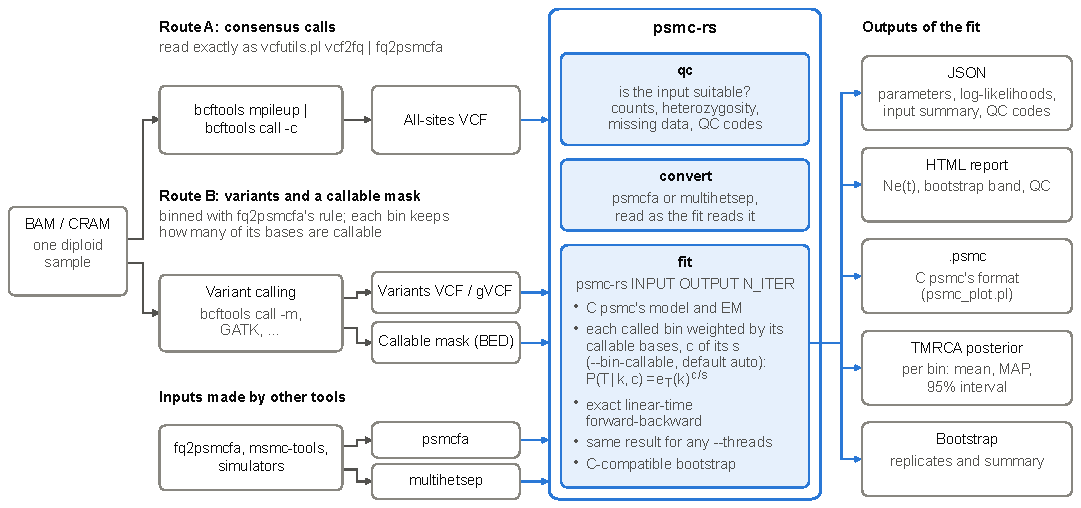
\includegraphics[width=\linewidth]{FIG/figures/fig1_workflow.pdf}
\caption{From reads to a PSMC history with \psmcrs{}. Reads of one diploid sample reach \psmcrs{} by one of two routes: consensus calling of every site (route A: \texttt{bcftools mpileup | bcftools call -c}, whose all-sites VCF \psmcrs{} reads as \texttt{vcfutils.pl vcf2fq | fq2psmcfa} would, byte for byte with the same depth limits) or variant calls with a callable mask (route B: bins made with \texttt{fq2psmcfa}'s rule, each called bin keeping the number of its bases that the mask calls callable). \texttt{psmcfa} and multihetsep files made by other tools are read as they are. \opt{psmc-rs qc} reports how suitable an input is, and \opt{psmc-rs convert} writes it as \texttt{psmcfa} or multihetsep. The fit (\opt{psmc-rs INPUT OUTPUT N\_ITER}) fits C psmc's model with each called bin weighted by its callable bases (\opt{--bin-callable auto}, the default: a homozygous bin with $c$ of its $s$ bases callable has probability $e_T(k)^{c/s}$ in state $k$) and writes the parameters (JSON), an HTML report and, on request, C psmc's \texttt{.psmc} output, per-bin summaries of the TMRCA's posterior and bootstrap replicates. \psmcrs{}'s own steps are blue; inputs, outputs and other tools are grey.}
\label{fig:workflow}
\end{figure}

\subsection*{\psmcrs{} reproduces C psmc on simulated genomes}

We simulated \EoneReps{} genomes of \EoneGenomeMb{}~Mb (\EoneChroms{} chromosomes of \EoneChromMb{}~Mb) under each of \EoneModelsW{} demographic models (constant size, a bottleneck, an expansion and the zigzag model of \citealt{schiffels2014}) and fitted each with both programs, with the pattern and maximum time that \citet{li2011} used for human genomes (Methods). The two programs estimated the truth equally well (Fig.~\ref{fig:sim}a--d and i, Table~\ref{tab:accuracy}): over the informative window, the 1\% to 99\% quantiles of the pairwise coalescence time, the RMSE of $\log_{10}\Ne$ against the truth averaged \EoneConstantTruthC{}, \EoneBottleneckTruthC{}, \EoneExpansionTruthC{} and \EoneZigzagTruthC{} for C psmc and \EoneConstantTruthRs{}, \EoneBottleneckTruthRs{}, \EoneExpansionTruthRs{} and \EoneZigzagTruthRs{} for \psmcrs{}.

Compared interval by interval, the programs' curves differed by an RMSE of \EoneRsCRmseMin{} to \EoneRsCRmseMax{} in $\log_{10}\Ne$ (median \EoneRsCRmseMedian{}), and no interval inside the window differed by more than \EoneRsCMaxAbs{} (Fig.~\ref{fig:sim}e--i). The scaled mutation and recombination rates and the time of the last interval agreed within a relative \EoneParamRelMax{}, and the log-likelihoods within \EoneLoglikeRelMax{} at every iteration and \EoneLoglikeLastRelMax{} at the last one both programs report. At the shared starting point, the first E-step's log-likelihoods agreed to a relative \EoneLoglikeFirstRelMax{}, so the two programs compute the same likelihood, and the differences arise in the iterations that follow. A diagnostic on a test genome (Methods) traced them not to the M-step's optimizer but to C psmc's expected counts: where the curves were \DiagCurve{} apart, a port of C psmc's Hooke--Jeeves search into \psmcrs{} left them \DiagHookeJeeves{} apart, whereas leaving the last bin of each sequence out of \psmcrs{}'s expected counts, as C psmc does, brought them within \DiagLastBin{}. Outside the window, where the data say little, the programs can disagree more: in \EoneAnyModel{} replicate~\EoneAnyReplicate{}, the first free $\lambda$, the relative size of the four most recent intervals (before \EoneRunawayKy{}~ky), ran away in both programs: \psmcrs{}'s stopped at its upper bound of $10^4$, and C psmc's, whose search is unbounded, reached \EoneRunawayC{} (an \Ne{} of \EoneRunawayCNe{}), \EoneAnyMax{} units of $\log_{10}\Ne$ apart. The next largest difference in any interval, inside or outside the window, was \EoneAnySecond{}. The log-likelihood never decreased from one iteration to the next, in \EoneMonotoneRuns{} of the \EoneRuns{} fits (Fig.~S1).

\begin{figure}[tbp]
\centering
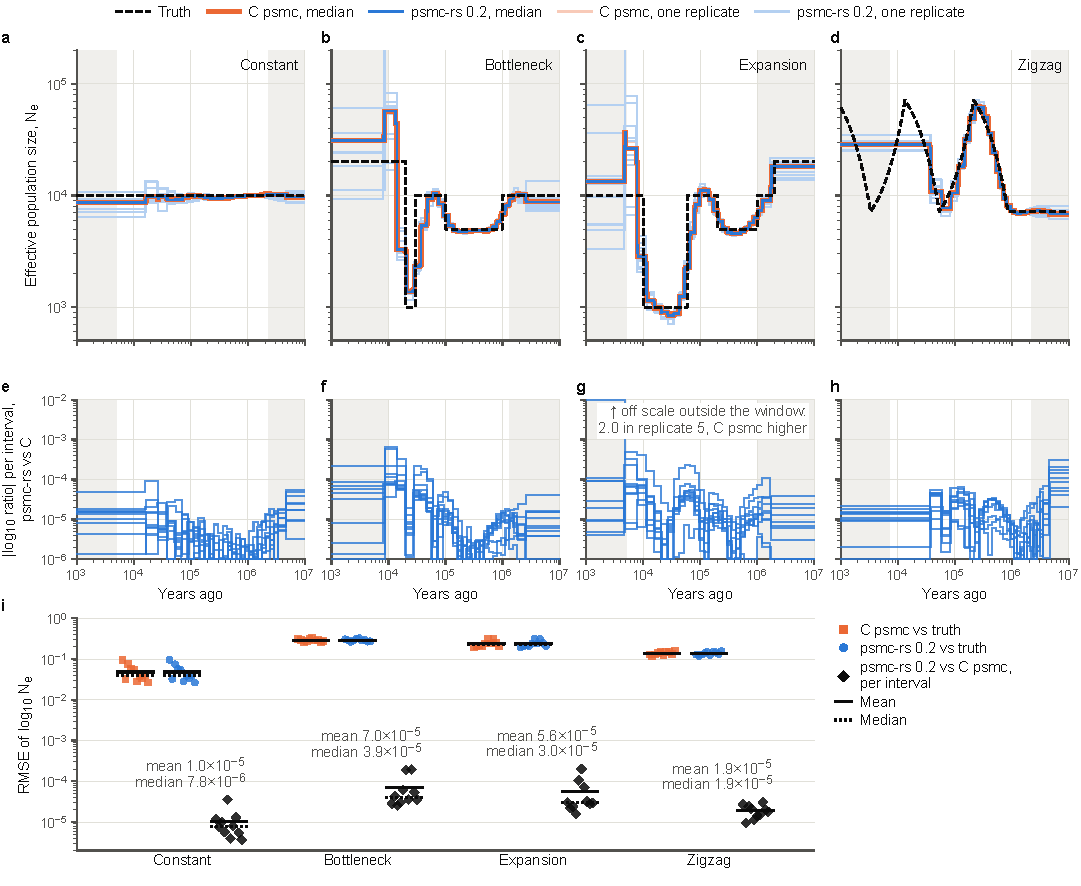
\includegraphics[width=\linewidth]{E1/figures/fig2_simulated_accuracy.pdf}
\caption{Accuracy on simulated genomes, and the two programs compared (E1). (a--d) One panel per model: the true $\Ne(t)$ (black, dashed), the fit of every replicate by C psmc (orange) and \psmcrs{} 0.2 (blue), thin and in a light tint, \psmcrs{}'s drawn over C psmc's, which they hide where the two coincide, and the pointwise median of each program's fits (C psmc drawn wider, underneath). Times outside the model's informative window, where no metric is computed, are shaded; fits outside the window can leave the panel. In \EoneAnyModel{} replicate~\EoneAnyReplicate{}, both programs' first free $\lambda$ (intervals 0--3, before \EoneRunawayKy{}~ky) ran away, \psmcrs{}'s to its upper bound of $10^4$ and C psmc's, unbounded, to \EoneRunawayC{} (an \Ne{} of \EoneRunawayCNe{}); both curves leave panel c there. (e--h) $|\log_{10}(\Ne^{\text{\psmcrs}}/\Ne^{\text{C}})|$ interval by interval for every replicate, on C psmc's intervals (log scale; smaller values are drawn on the axis floor); a larger difference outside the window is named in the panel. (i) RMSE of $\log_{10}\Ne$ on the informative window, per replicate: each program against the truth (on 200 log-spaced times) and \psmcrs{} against C psmc (interval by interval, each interval weighted by its log-time width in the window), with the mean (solid) and median (dotted) of each group. Simulations: $\mu=2.5\times10^{-8}$ per bp per generation, $g=25$ years.}
\label{fig:sim}
\end{figure}

\begin{table}[tbp]
\centering\small
\caption{Accuracy and equivalence on simulated genomes (E1). For each model, \EoneReps{} genomes of \EoneGenomeMb{}~Mb: the informative window in years, the RMSE of $\log_{10}\Ne$ against the truth on it (mean $\pm$ SD over replicates), and the difference between the programs interval by interval (median over replicates of the RMSE, and the largest absolute difference in any interval of the window).}
\label{tab:accuracy}
\begin{tabular}{lrrrrrr}
\toprule
& \multicolumn{2}{c}{Window (years)} & \multicolumn{2}{c}{RMSE vs truth} & \multicolumn{2}{c}{psmc-rs vs C psmc} \\
\cmidrule(lr){2-3}\cmidrule(lr){4-5}\cmidrule(lr){6-7}
Model & from & to & C psmc & psmc-rs & RMSE (median) & max $|\Delta|$ \\
\midrule
constant & 5,025 & 2,302,585 & 0.048 $\pm$ 0.023 & 0.048 $\pm$ 0.023 & \ensuremath{7.8\times10^{-6}} & \ensuremath{9.2\times10^{-5}} \\
bottleneck & 10,050 & 1,322,585 & 0.291 $\pm$ 0.021 & 0.291 $\pm$ 0.021 & \ensuremath{3.9\times10^{-5}} & \ensuremath{6.6\times10^{-4}} \\
expansion & 5,025 & 1,052,585 & 0.240 $\pm$ 0.043 & 0.240 $\pm$ 0.043 & \ensuremath{3.0\times10^{-5}} & \ensuremath{4.8\times10^{-4}} \\
zigzag & 7,141 & 2,167,766 & 0.138 $\pm$ 0.013 & 0.138 $\pm$ 0.013 & \ensuremath{1.9\times10^{-5}} & \ensuremath{6.6\times10^{-5}} \\
\bottomrule
\end{tabular}

\end{table}

\subsection*{Real genomes: a human and three turtles}

We fitted both programs to four real genomes (Fig.~\ref{fig:real}): NA12878's \EtwoHumanSequences{} autosomes from the high-coverage 1000 Genomes data (the input E7 makes for that genome) and three side-necked turtles, \textit{Emydura subglobosa}, \textit{Hydromedusa tectifera} and \textit{Pelusios castaneus}, whose \texttt{psmcfa} files hold \EtwoTurtleSeqMin{} to \EtwoTurtleSeqMax{} sequences. The curves agreed to an RMSE of \EtwoRsCRmseMin{} to \EtwoRsCRmseMax{} in $\log_{10}\Ne$, with no interval of the window more than \EtwoRsCMaxAbs{} apart; the parameters agreed within a relative \EtwoParamRelMax{}, the log-likelihoods at the last iteration both report within \EtwoLoglikeRelMax{} and the first E-step's within \EtwoLoglikeFirstRelMax{}. The RMSE was smallest for NA12878, with \EtwoHumanSequences{} sequences, and largest for \textit{P. castaneus}, with \EtwoTurtleSeqMax{}, consistent with the sequences' last bins causing the difference. The bootstrap of each genome by \psmcrs{} (\EtwoBootReps{} replicates of 50~Mb blocks on \EtwoBootThreads{} threads) refitted the main fit exactly, every parameter, log-likelihood and iteration count equal to those of the genome's one-thread fit, and its 95\% bands, whose median width over the window was \EtwoBandWidthMin{} to \EtwoBandWidthMax{} in $\log_{10}\Ne$, held both programs' curves at each of 200 log-spaced times in the window. \psmcrs{}'s \opt{qc} flagged \EsixSaturatedW{} of the turtle genomes for bin saturation, with \EsixSatShareLo{} to \EsixSatShareHi{} of their heterozygous bins likely to hold more than one heterozygous site, and recommended bins of \EsixSatBinLo{} to \EsixSatBinHi{}~bp; it also flagged all \EsixShortSeqW{} turtle genomes for sequences shorter than the bootstrap's blocks (Table~S1).

Under the pattern \opt{4+25*2+4+6}, whose first free $\lambda$ spans four intervals, all \EtwoPeaksDefaultW{} turtle curves rose to a recent peak \EtwoPeakMin{} to \EtwoPeakMax{} times the plateau that preceded it, the shape that \citet{hilgers2025} showed to be an artefact in many published PSMC curves. Splitting that first window into two or four free $\lambda$s removed the peak in all \EtwoSplitFitsW{} fits (Fig.~S7), increased the log-likelihood by \EtwoSplitGainMin{} to \EtwoSplitGainMax{} units, and changed the older history little, by an RMSE of at most \EtwoSplitOlderMax{} in $\log_{10}\Ne$ at the same times. The bootstrap did not expose the peaks: by the same rule, \EtwoBootPeakHyd{} of the \EtwoBootReps{} replicates of \textit{H. tectifera}, \EtwoBootPeakPel{} of \textit{P. castaneus}'s and \EtwoBootPeakEmy{} of \textit{E. subglobosa}'s had one.

\begin{figure}[tbp]
\centering
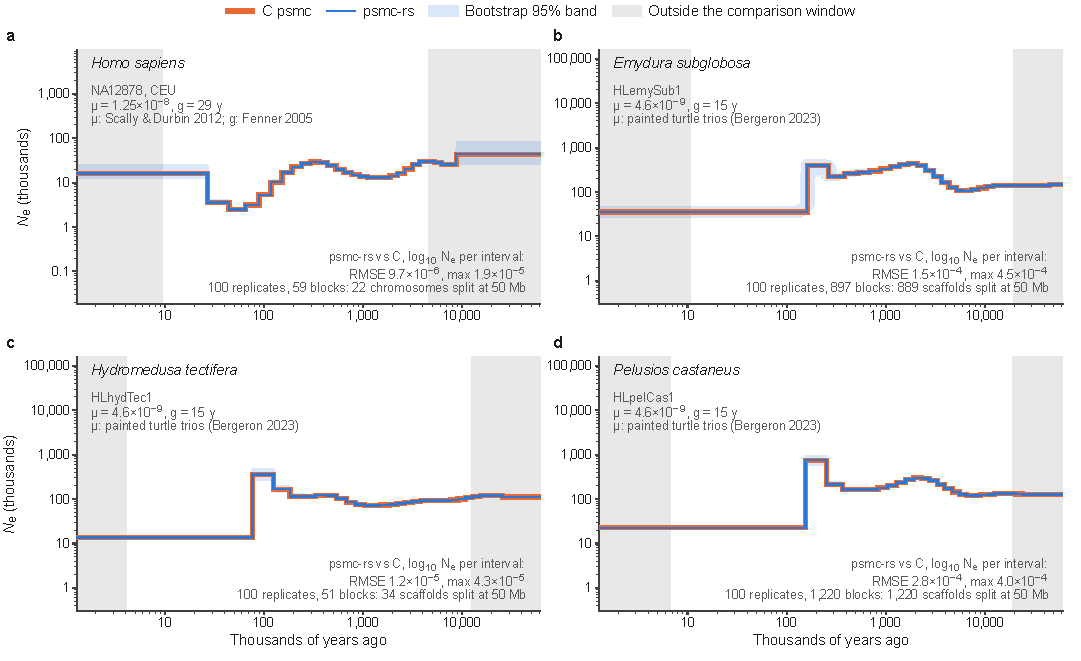
\includegraphics[width=\linewidth]{E2/figures/fig3_real_genomes.pdf}
\caption{Four real genomes fitted by C psmc and \psmcrs{} (E2). One panel per genome: C psmc's fit (orange, wider, underneath), \psmcrs{}'s (blue) and the pointwise 95\% band of \psmcrs{}'s bootstrap (\EtwoBootReps{} replicates; light blue). The bootstrap resamples blocks of 50~Mb (\texttt{splitfa}'s: a remainder shorter than 1.5 blocks stays in the last block, so a sequence shorter than 1.5 blocks is one block); each panel gives its genome's blocks and sequences. Each genome is scaled with its own mutation rate and generation time: the turtles with $\mu=4.6\times10^{-9}$ per bp per generation, the mean germline rate of nine trios of the painted turtle \textit{Chrysemys picta} \citep{bergeron2023}, as no side-necked turtle's rate has been measured, and $g=15$ years, close to the generation times of two of the species \citep{sozzoni2025}; NA12878 with $\mu=1.25\times10^{-8}$ \citep{scally2012} and $g=29$ years \citep{fenner2005}. \Ne{} and time scale as $1/\mu$, and time also as $g$. Times outside the window on which the programs are compared (1\% to 99\% of pairwise coalescence times under C psmc's fit) are shaded; each panel gives the RMSE between the programs over the window, interval by interval, and the largest difference. The turtles' recent peaks are artefacts of the pattern's first window (Fig.~S7).}
\label{fig:real}
\end{figure}

\subsection*{Speed, memory and determinism}

We timed both programs and \psmcrs{}'s first release, 0.1, on constant-size genomes of 1, 3, 10 and 30 chromosomes of 100~Mb, each run alone on an exclusive node, with \EthreeRepeatsW{} repeats on \EthreeNodesW{} nodes of one CPU model (\EthreeCpu{}; Table~\ref{tab:timing}, Fig.~\ref{fig:perf}). All \EthreeRuns{} timed runs passed the protocol's checks for interference (Methods), and in every setup but one the fastest and slowest repeats were within \EthreeSpreadMaxMost{} of the median. On \EthreeBigMb{}~Mb, 25 iterations took C psmc \EthreeCWall{}~s (\EthreeCMin{} minutes) and \psmcrs{} \EthreeRsOneWall{}~s on one thread, \EthreeSpeedOne{} times as fast (\EthreeSpeedOneMin{} to \EthreeSpeedOneMax{} at every size); \psmcrs{} 0.1 took \EthreeRsZeroWall{}~s. \psmcrs{} runs the E-step of each sequence on one thread and processes the sequences in parallel: on \EthreeBigMb{}~Mb it was \EthreeSpeedEight{}, \EthreeSpeedSixteen{} and \EthreeSpeedThirty{} times as fast as C psmc on 8, 16 and 30 threads. Its parallel efficiency on 2 to 30 threads was \EthreeEffMin{} to \EthreeEffMax{}, close to the \EthreeEffCap{} to 1 that whole chromosomes per thread allow (Fig.~S4). The longest sequence bounds the speed-up: one 100~Mb chromosome took \EthreeChromWallMin{} to \EthreeChromWallMax{}~s on 1, 8 and 30 threads, and every setup took \EthreeRoundMin{} to \EthreeRoundMax{}~s per round of chromosomes on its threads. Peak memory was \EthreeRsMemOne{}~MB on one thread and \EthreeRsMemThirty{}~MB on 30, against \EthreeCMem{}~MB for C psmc and \EthreeRsZeroMemOne{} to \EthreeRsZeroMemThirty{}~MB for \psmcrs{} 0.1, because \psmcrs{} keeps the forward pass only at checkpoints and recomputes the rest (Methods).

\psmcrs{}'s output does not depend on the number of threads. At each genome size, its fitted models (JSON) from every thread count, repeat and node, \EthreeDetRsTotal{} outputs in all, were byte-identical, as were C psmc's \EthreeDetCTotal{} \texttt{.psmc} outputs. \psmcrs{} 0.1's output depended on whether it ran on one thread or several: on genomes of more than one chromosome, its outputs on 8 and 30 threads, identical to each other, differed from its one-thread output by up to a relative \EthreeRsZeroDiffMax{} in the parameters (\EthreeDetRsZeroIdentical{} of its \EthreeDetRsZeroTotal{} outputs identical to the one-thread output). On a real genome, NA12878's bootstrap, run with one seed on \EtwoBootThreads{} threads in E2 and on \EsevenBootThreads{} in E7, wrote \EsevenBootFilesIdentical{} of \EsevenBootFiles{} files byte for byte the same.

\begin{figure}[tbp]
\centering
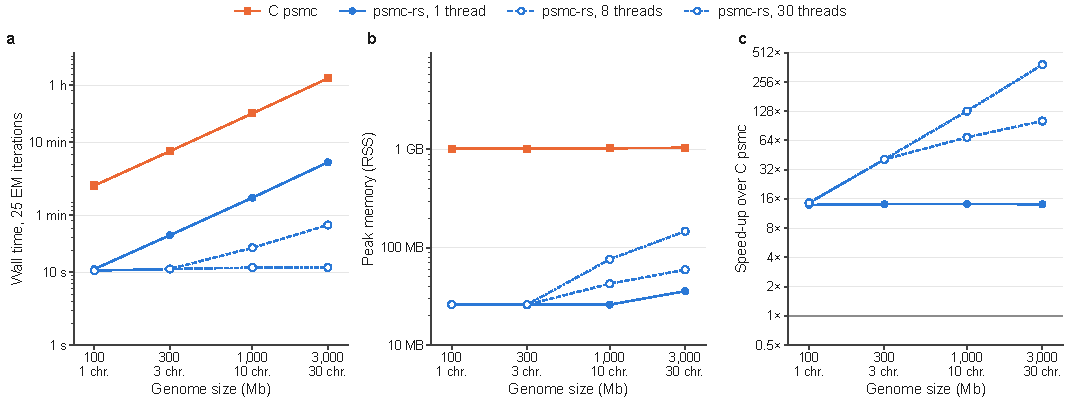
\includegraphics[width=\linewidth]{E3/figures/fig4_performance.pdf}
\caption{Run time, memory and speed-up (E3). Every run fits 25 EM iterations to a constant-size genome of 100~Mb chromosomes (1, 3, 10 and 30 chromosomes; second line of each tick label), alone on an exclusive node; lines and markers are medians over \EthreeRepeatsW{} repeats on \EthreeNodesW{} nodes, and small dots, mostly hidden by the markers, individual repeats. (a) Wall time: C psmc (one thread), \psmcrs{} 0.1 and \psmcrs{} 0.2 on 1, 8 and 30 threads (solid, dashed and dash-dotted). (b) Peak memory, the larger of the program's \texttt{ru\_maxrss} and the sampled peak of its process tree; for \psmcrs{} 0.2 below 1,000~Mb this is an upper bound (Supplementary Note~1, section~10). (c) Speed-up over C psmc, the ratio of the medians. \psmcrs{} runs the E-step of each sequence on one thread, in parallel across sequences, so on $t$ threads a genome of $n$ equal chromosomes takes about $\lceil n/t\rceil$ times one chromosome's time: threads beyond the number of chromosomes add nothing, and the 30-thread speed-up on \EthreeBigMb{}~Mb holds because each of its 30 chromosomes has a thread. On a real genome, the longest sequence sets the bound.}
\label{fig:perf}
\end{figure}

\begin{table}[tbp]
\centering\small
\caption{Run time and memory (E3). Median wall time of 25 EM iterations over \EthreeRepeatsW{} repeats on exclusive \EthreeCpu{} nodes, for constant-size genomes of 100~Mb chromosomes; speed-up over C psmc and peak memory (median, MB of $2^{20}$ bytes) on \EthreeBigMb{}~Mb. -- marks a setup not timed. \psmcrs{} 0.1 ran without smoothing and with M-steps of up to 1,000 iterations, as \psmcrs{} 0.2 does (Methods). The memory at the other sizes is given in Supplementary Note~1, section~10.}
\label{tab:timing}
\begin{tabular}{lrrrrrrr}
\toprule
& & \multicolumn{4}{c}{Wall time, median (s)} & \multicolumn{2}{c}{3,000 Mb} \\
\cmidrule(lr){3-6}\cmidrule(lr){7-8}
Tool & Threads & 100 Mb & 300 Mb & 1,000 Mb & 3,000 Mb & Speed-up & Memory (MB) \\
\midrule
C psmc & 1 & 152.5 & 449.4 & 1,478.3 & 4,455.9 & 1 & 1,062 \\
psmc-rs & 1 & 11.0 & 31.8 & 103.9 & 317.0 & 14 & 36 \\
psmc-rs & 2 & -- & -- & -- & 163.3 & 27 & 39 \\
psmc-rs & 4 & -- & -- & -- & 87.3 & 51 & 47 \\
psmc-rs & 8 & 10.5 & 11.0 & 21.5 & 43.9 & 101 & 59 \\
psmc-rs & 16 & -- & -- & -- & 22.5 & 198 & 88 \\
psmc-rs & 30 & 10.5 & 11.0 & 11.5 & 11.5 & 386 & 148 \\
\bottomrule
\end{tabular}

\end{table}

\subsection*{Partly callable bins bias PSMC, and weighting each bin by its callable bases corrects it}

To measure how missing data affect PSMC, we made \EfourRepsW{} simulated \EfourGenomeMb{}~Mb bottleneck genomes partly uncallable in two patterns, each covering 10\% or 30\% of positions: clustered, in uncallable runs of \EfourClusRunKb{}~kb on average, and dispersed, in runs of \EfourDispRunBp{}~bp (Fig.~\ref{fig:inputs}). The standard route, a consensus sequence converted by \texttt{fq2psmcfa} and fitted with C psmc's model, gave the same bins and the same fit as \psmcrs{} with every called bin taken as full (Methods). With clustered masks whole bins went missing, and both this route and \psmcrs{}'s weighting stayed close to the complete-data fit, their scaled mutation rates ($\theta$) \EfourClusThirtyFqTheta{} and \EfourClusThirtyAutoTheta{} low with 30\% missing. With dispersed masks most called bins kept only part of their bases (\EfourDispTenPartly{} of them with 10\% missing, \EfourDispThirtyPartly{} with 30\%), and taking such bins as full made $\theta$ low by \EfourDispTenFqTheta{} (10\% missing) and \EfourDispThirtyFqTheta{} (30\%), and every time and size with it: the curves lay \EfourDispTenFqRmse{} and \EfourDispThirtyFqRmse{} from the complete-data fit (RMSE of $\log_{10}\Ne$). Weighting each called bin by its callable bases (Methods) reduced the bias in $\theta$ to \EfourDispTenAutoTheta{} and \EfourDispThirtyAutoTheta{}, and the distance from the complete-data fit to \EfourDispTenAutoRmse{} and \EfourDispThirtyAutoRmse{}. MSMC's multihetsep format, which does not record where the uncalled sites of an interval lie, was biased as well ($\theta$ \EfourDispTenMhsTheta{} and \EfourDispThirtyMhsTheta{} low with 10\% and 30\% dispersed missing), and so was a VCF read without its mask, which counts every uncallable site as homozygous (\EfourDispThirtyNomaskTheta{} with 30\% dispersed and \EfourClusThirtyNomaskTheta{} with 30\% clustered missing). Dispersed missing data are common in real masks: in the 1000 Genomes inputs below, \EsevenPartly{} of each genome's called bins had some uncallable bases.

\begin{figure}[tbp]
\centering
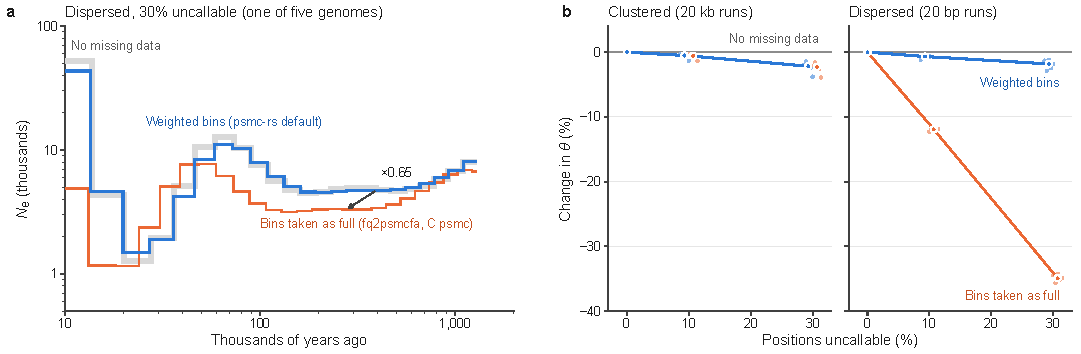
\includegraphics[width=\linewidth]{E4/figures/fig5_input_preparation.pdf}
\caption{Partly callable bins bias PSMC, and \psmcrs{}'s per-bin weighting removes most of the bias (E4). Bottleneck genomes of \EfourGenomeMb{}~Mb (\EfourRepsW{} replicates) with no missing data, or with 10\% or 30\% of positions uncallable in clustered (mean \EfourClusRunKb{}~kb) or dispersed (mean \EfourDispRunBp{}~bp) runs. Routes: \psmcrs{} on the VCF with its callable mask, each called bin weighted by its callable bases (\opt{--bin-callable auto}, the default; blue); the same bins with every called bin taken as full (\opt{--bin-callable ignore}; dark blue, dashed), which is what \texttt{fq2psmcfa} and C psmc do (the consensus FASTA $\to$ \texttt{fq2psmcfa} route gives the same bins and the same fit and is not drawn separately); multihetsep (yellow), read back with its uncalled sites placed at the start of each interval; and the VCF read without its mask (pink). (a) $\theta$ per bin relative to the complete-data fit of the same genome. (b) RMSE of $\log_{10}\Ne$ against the truth on the informative window. (c) RMSE of $\log_{10}\Ne$ against the complete-data fit, exact over log time on the window. In a--c, dots are replicates and bars their means. (d) The curves of one replicate with the 30\% dispersed mask, its complete-data fit (grey) and the truth; times outside the informative window are shaded. (e, f) Bias over time, the mean over replicates of $\log_{10}(\Ne/\Ne^{\text{true}})$, with the 30\% clustered and dispersed masks; grey, the complete data. Simulations: $\mu=2.5\times10^{-8}$ per bp per generation, $g=25$ years.}
\label{fig:inputs}
\end{figure}

\subsection*{What the bootstrap bands measure}

To calibrate the bootstrap we simulated \EfiveFits{} independent genomes of \EfiveGenomeMb{}~Mb (\EfiveChromsW{} chromosomes) under the bottleneck model and fitted each: the spread of their fits at each time is the true sampling distribution of the estimate. We then bootstrapped \EfiveDatasets{} of the genomes with \EfiveReps{} replicates each, with \texttt{splitfa}'s default blocks of 50~Mb (\EfiveFiftyTrunks{} per genome) and with the 5~Mb blocks that \citet{li2011} used (\EfiveFiveTrunks{} per genome; Fig.~\ref{fig:boot}). The bootstrap's standard deviation of $\log_{10}\Ne$ was a median of \EfiveFiftySd{} times the true one with 50~Mb blocks (95\% CI \EfiveFiftySdLo{}--\EfiveFiftySdHi{}) and \EfiveFiveSd{} times with 5~Mb blocks (\EfiveFiveSdLo{}--\EfiveFiveSdHi{}). The 95\% bands covered the mean of the independent fits at \EfiveFiftyCovMean{} (50~Mb) and \EfiveFiveCovMean{} (5~Mb) of the times in the window, but the true \Ne{} at only \EfiveFiftyCov{} (\EfiveFiftyCovLo{}--\EfiveFiftyCovHi{}) and \EfiveFiveCov{} (\EfiveFiveCovLo{}--\EfiveFiveCovHi{}). The shortfall is PSMC's bias, not the bootstrap's spread: the fits' median absolute bias, \EfiveBias{} in $\log_{10}\Ne$, was about twice their true standard deviation, \EfiveSdTrue{}, and even the truth averaged over each free parameter's span, which is the most a PSMC curve can represent, was covered at only \EfiveFiftyCovProj{} and \EfiveFiveCovProj{} of times. Bootstrap bands therefore describe how much an estimate would vary between genomes with the same history, which smaller blocks describe better; they are not confidence intervals for the history.

\begin{figure}[tbp]
\centering
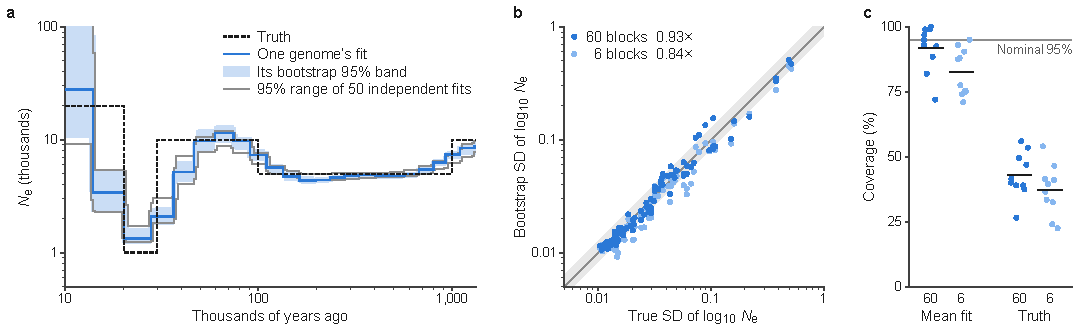
\includegraphics[width=\linewidth]{E5/figures/fig6_bootstrap_calibration.pdf}
\caption{Calibration of the bootstrap (E5). \EfiveFits{} independent bottleneck genomes of \EfiveChroms{}$\times$50~Mb, each fitted once, give the true sampling distribution of the estimate; \EfiveDatasets{} of them are bootstrapped (\EfiveReps{} replicates) with blocks of 50~Mb (blue) and 5~Mb (dark blue, dashed). Every panel spans the model's informative window. (a) One genome: the truth (dashed), the 95\% range of the independent fits (grey), the genome's fit (blue) and the edges of its bootstrap 95\% bands. (b) Standard deviation of $\log_{10}\Ne$: the true one over the independent fits (black, with its $\chi^2$ 95\% interval, light grey) and the bootstrap's (median over the bootstrapped genomes). (c) Bootstrap SD over true SD: median over genomes and interquartile range; the light grey band is where a bootstrap whose SD equalled the true one would fall, given the true SD's own sampling error. (d) Share of the bootstrapped genomes whose 95\% band covers the true \Ne{} (thick; Clopper--Pearson 95\% interval for 50~Mb blocks) and the fits' geometric mean (thin), against the nominal 95\%; with \EfiveDatasets{} genomes the share moves in steps of 10\%. (e) The same share for each genome's pattern-projected truth, the truth averaged over each free parameter's span. One-point spikes in b--e are times at which the fits' interval boundaries, which move with each fit's $\theta$ and maximum time, straddle the grid time. The legend gives each block size's coverage averaged over the window, with intervals from resampling the bootstrapped genomes. Simulations: $\mu=2.5\times10^{-8}$ per bp per generation, $g=25$ years.}
\label{fig:boot}
\end{figure}

\subsection*{Input formats agree, and the posterior TMRCA is calibrated}

Read as a VCF, each of \EoneModelsW{} simulated genomes (one per model of E1) gave the same bins and the same fit, value for value, as its \texttt{psmcfa} file. Read as multihetsep, which ends at a sequence's last heterozygous site, it lost the \EsixMhsTailMin{} to \EsixMhsTailMax{} bins that follow those sites but no other bin differed, and the fits moved by at most \EsixMhsMaxAbs{} in $\log_{10}\Ne$ (Fig.~S2). Decoding a bottleneck genome bin by bin with its fitted model, the posterior mean TMRCA correlated with the true TMRCA at $r=$~\EsixDecodeR{} on a log scale over \EsixDecodeBins{} bins, and the PSMC states holding the central 95\% of the posterior held the true TMRCA in \EsixDecodeCov{} of bins (Fig.~S3). By decile of the true TMRCA this coverage ranged from \EsixTrueDecileMin{} to \EsixTrueDecileMax{}, the posterior mean being too old by \EsixYoungBias{} in $\log_{10}$ on average for the youngest decile and too young by \EsixOldBias{} for the oldest; by decile of the posterior mean, which is what an analysis sees, it ranged from \EsixPostDecileMin{} to \EsixPostDecileMax{}.

\subsection*{2,504 high-coverage human genomes}

We applied \psmcrs{} to all \EsevenGenomes{} unrelated individuals of the high-coverage 1000 Genomes data \citep{byrskabishop2022}: \EsevenPops{} populations of \EsevenPerPopMin{} to \EsevenPerPopMax{} individuals, sequenced to a median depth of \EsevenDepth{}$\times$ (Fig.~\ref{fig:kg}). From the joint-called VCFs of chromosomes 1--22 (\EsevenRecords{} records, \EsevenVcfTb{}~TB) we made one input per genome with the strict accessibility mask, and with the position of every record that failed the callset's filters (\EsevenNonpass{} records) set missing: a median of \EsevenCallableGb{}~Gb of callable sequence per genome (Methods). For \EsevenPilotSamplesW{} individuals, chromosome~\EsevenPilotChrom{} converted directly from the joint VCF gave byte-identical files. Against Genome in a Bottle's benchmark for NA12878 \citep{zook2019,wagner2022}, the heterozygous single-nucleotide sites of its input, the callset's PASS records read with \psmcrs{}'s rule, had a precision of \EsevenGiabPrecision{} and a recall of \EsevenGiabRecall{}, over \EsevenGiabTruth{} benchmark sites in \EsevenGiabMb{}~Mb inside both the strict mask and the benchmark's regions; of the \EsevenGiabFn{} sites missed, \EsevenGiabFnIndel{} lay at records the callset gave as heterozygous for an allele other than a single nucleotide (an indel or a spanning deletion) and \EsevenGiabFnNonpass{} at records that failed its filters.

With one fit per thread on a shared node, \psmcrs{} took a median of \EsevenRsFitMin{} minutes per genome, \EsevenRsCoreHours{} core-hours for the cohort. C psmc, run the same way on a default set of \EsevenDefault{} genomes (two per population, including NA18507 and NA19239, two of the genomes that \citeauthor{li2011} analysed, and NA12878), took a median of \EsevenCFitMin{} minutes per genome, which would make about \EsevenCCoreHoursAll{} core-hours for the cohort; these are costs on a shared node, and E3 measures speed. On those \EsevenDefault{} genomes the two programs' curves agreed to an RMSE of \EsevenRsCRmseMin{} to \EsevenRsCRmseMax{} in $\log_{10}\Ne$, at most \EsevenRsCMaxAbs{} in any interval of the window (three of them in Fig.~\ref{fig:kg}g--i). No fit of the \EsevenGenomes{} genomes reached \psmcrs{}'s bound on the size parameters. \psmcrs{}'s bootstraps of NA18507, NA19239 and NA12878 (\EsevenBootReps{} replicates) took a median of \EsevenBootMin{} minutes each on \EsevenBootThreads{} threads, refitted their main fits exactly, and held both programs' curves.

The population histories (Fig.~\ref{fig:kg}a--f, Fig.~S5) have the features of published single-genome PSMC analyses of human genomes \citep{li2011,prufer2014,mallick2016}. The median curves of the four superpopulations outside Africa fell to \EsevenNonAfrMinNeLo{} to \EsevenNonAfrMinNeHi{} between \EsevenNonAfrMinKyLo{} and \EsevenNonAfrMinKyHi{} thousand years ago, while the African median declined only to \EsevenAfrMinNe{}, \EsevenAfrMinKy{} thousand years ago. From \EsevenConvergeKy{} thousand years ago to the end of the window, \EsevenWindowHiMy{} million years ago, the five superpopulations' median curves were within 20\% of one another, with a local maximum of \EsevenHumpNeLo{} to \EsevenHumpNeHi{} between \EsevenHumpKyLo{} and \EsevenHumpKyHi{} thousand years ago, a feature that ancestral population structure can produce without any change in size \citep{mazet2016,cousins2025}. Heterozygosity was \EsevenHetAfr{} per callable kb in African and \EsevenHetEas{} in East Asian genomes (medians; Fig.~S6a). Splitting the first time window into its four intervals, the check that removed the turtles' peaks, changed the human curves by a median RMSE of \EsevenSplitRmse{} between corresponding intervals and left their recent rise, where there was one, in place (Fig.~S6c); in \EsevenSplitBoundW{} of the \EsevenSplitN{} split fits one recent interval reached the bound, as one genome barely constrains such short intervals.

Fig.~\ref{fig:kg} shows fits of the \texttt{psmcfa} files, which record no callable bases per bin and are therefore fitted with C psmc's model, comparable with C psmc and with published curves. The same \EsevenDefault{} genomes fitted from their VCFs, each bin weighted by its callable bases, gave a $\theta$ \EsevenThetaShift{} higher (\EsevenThetaShiftLo{} to \EsevenThetaShiftHi{}), close to the \EsevenThetaExpected{} expected from the \EsevenMissingShare{} of the called bins' bases that were uncallable, and curves \EsevenNeShift{} higher in $\log_{10}\Ne$ on average at the same times, with the populations' order and shapes unchanged (Figs~S5 and S6b). The \texttt{psmcfa} inputs and the fits of all \EsevenGenomes{} genomes are released as a resource (Data availability).

\begin{figure}[tbp]
\centering
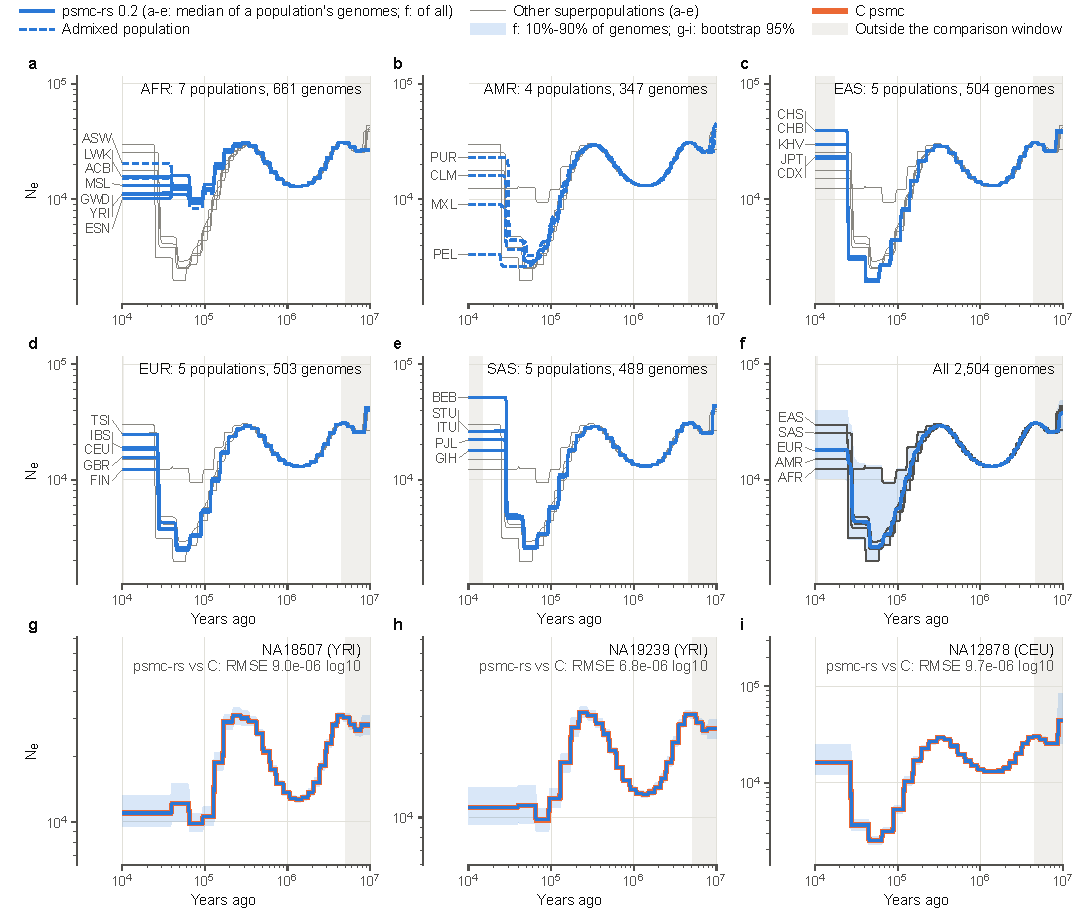
\includegraphics[width=\linewidth]{E7/figures/fig7_1000_genomes.pdf}
\caption{\psmcrs{} on the \EsevenGenomes{} unrelated high-coverage genomes of the 1000 Genomes Project (E7). (a--e) One panel per superpopulation: each population's curve is the median of its genomes' fits (\EsevenPerPopMin{} to \EsevenPerPopMax{} genomes per population), blue, admixed populations dashed; the other superpopulations' medians are grey hairlines. Fig.~S5 gives each population's spread between its genomes. (f) Every genome of the cohort: the median of all (blue) with the spread between individuals (10\% to 90\%; a band of individuals, not a confidence interval) and each superpopulation's median. Panels a--f share one \Ne{} axis. These are fits of the \texttt{psmcfa} files, which take every called bin as full; the VCF route gave a $\theta$ \EsevenThetaShift{} higher on the \EsevenDefault{} default genomes (Fig.~S6b), a shift that leaves the populations' order and shapes as they are. (g--i) NA18507 and NA19239, two of the genomes that \citet{li2011} analysed, and NA12878: \psmcrs{} (blue) over C psmc (orange, wider, underneath) on the same \texttt{psmcfa}, with \psmcrs{}'s bootstrap band; the note gives the RMSE between the programs, interval by interval. Times outside the comparison window (1\% to 99\% of pairwise coalescence times; for a group, the median of its genomes' windows) are shaded. Curves are scaled with $\mu=\EsevenMu$ per bp per generation and $g=\EsevenG$ years.}
\label{fig:kg}
\end{figure}

\FloatBarrier
\section*{Discussion}

\psmcrs{} makes PSMC fast enough for population-scale data while keeping its results comparable with those of the original program. Fitted to the same input, its curves differ from C psmc's by much less than the method's own error: by an RMSE of at most \EoneRsCRmseMax{} in $\log_{10}\Ne$ over the informative window on simulated genomes, against errors of \EoneConstantTruthRs{} to \EoneBottleneckTruthRs{} relative to the truth and a sampling standard deviation of \EfiveSdTrue{} between genomes of \EfiveGenomeMb{}~Mb with the same history. The residual difference traces mainly to C psmc's leaving each sequence's last bin out of its expected counts, and \psmcrs{}'s results do not depend on the number of threads. Analyses of the same input files can therefore move to \psmcrs{}, and repeat or extend published PSMC analyses, without their conclusions changing because of the program.

Three findings matter beyond the software. First, bins that are only partly callable bias PSMC by about the share of their bases that are missing, and real masks, such as the 1000 Genomes strict mask with the callset's filters, leave about a quarter of called bins in that state. Weighting each bin's probability by its callable bases follows the Poisson bin likelihood of cobraa and PSMC+ \citep{cousins2024,cousins2025} and brings it to the binary PSMC model that most analyses use, while leaving the model of complete data and of \texttt{psmcfa} files exactly C psmc's. The correction needs an input that records each bin's callable bases, such as a VCF with its mask; a \texttt{psmcfa} file does not, so curves fitted from such files have $\theta$, and with it every size and time, too low by roughly the share of bases missing from called bins; in the 1000 Genomes data the VCF route gave a $\theta$ \EsevenThetaShift{} higher. Second, for the bottleneck model and genome size we studied, the block bootstrap of PSMC measured sampling variation, not error: its bands covered the true history at fewer than half of the times, because the bias of PSMC's discretized estimate exceeded its sampling error. Other histories and longer genomes will shift that balance, but in none of them can the bootstrap see the bias. Smaller blocks than \texttt{splitfa}'s default calibrated the spread better. Bands should be read as describing how an estimate would vary between genomes, and features that the bootstrap supports, such as the recent peaks that every replicate of two of the turtles reproduced, still need to be checked against the model's discretization \citep{hilgers2025}. Third, single-genome PSMC applied to every individual of a high-coverage cohort reproduces the published picture of human history and gives, for each genome, a fit that can be compared with C psmc's and with other genomes'.

The model of \psmcrs{} is PSMC's, with its limits. One genome carries little information about the last few thousand generations, where the first free $\lambda$ is barely constrained and can run away; \psmcrs{} bounds it and warns when it reaches the bound. Bins of 100~bp saturate in genomes as diverse as the turtles', for which \psmcrs{}'s \opt{qc} recommends smaller bins. Ancestral population structure can produce changes in a single-genome curve that are not changes in size \citep{mazet2016,cousins2025}, and methods that combine many genomes, such as MSMC2 \citep{schiffels2020}, SMC++ \citep{terhorst2017} or PHLASH \citep{terhorst2025}, resolve recent times better and can give different histories for the same populations. \psmcrs{} does not replace them; it makes the single-genome reference fast, reproducible and correct for partly callable data. Finally, \psmcrs{}'s results are identical across thread counts but, as floating-point computations, differ slightly between platforms. Refitted on a laptop of another architecture, operating system and mathematical library (Supplementary Note~1, section~9), the \EoneGenomes{} simulated genomes gave parameters within a relative \XpRsParamMax{} and curves within an RMSE of \XpRsRmseMax{} in $\log_{10}\Ne$ of the cluster's, closer by a median factor of \XpRatioCMedian{} than two builds of C psmc on the same two machines were to each other, although no output was byte-identical.

\FloatBarrier
\section*{Methods}

\subsection*{The PSMC model as \psmcrs{} fits it}

\psmcrs{} fits the model of \citet{li2011} with the conventions of C psmc 0.6.5-r74 \citep{psmcC}. Time is measured in units of $2N_0$ generations and divided into $n+1$ intervals $[t_k,t_{k+1})$, with $t_k=\alpha(e^{\beta k}-1)$ for $k=0,\dots,n-1$, $\beta=\ln(1+t_{\max}/\alpha)/n$, $\alpha=0.1$, $t_n=t_{\max}$ and $t_{n+1}$ a large value standing for infinity (1,000, as in C psmc). The population size in interval $k$ is $\lambda_kN_0$. The free parameters are the scaled mutation rate $\theta$ and recombination rate $\rho$ per bin, $t_{\max}$, and the free $\lambda$s, each spanning consecutive intervals according to a pattern: \opt{4+25*2+4+6}, the setting of \citet{li2011} for human genomes used throughout this work, has 64 intervals and 28 free $\lambda$s, the first spanning the four most recent intervals. The hidden states are the intervals; the initial distribution, the transition probabilities and the expected coalescence time $\bar t_k$ within each interval are computed exactly as C psmc computes them (\psmcrs{}'s code is a line-by-line port of its \texttt{psmc\_update\_hmm}). A bin is heterozygous (K) if it holds at least one heterozygous site, homozygous (T) if it holds none, or missing (N), with emission probabilities $e_T(k)=e^{-\theta\bar t_k}$, $e_K(k)=1-e_T(k)$ and $e_N(k)=1$. Sizes and times are scaled to individuals and years with a mutation rate $\mu$ per bp per generation, the bin size $s$ and a generation time $g$: $N_0=\theta/(4\mu s)$, $\Ne=\lambda_kN_0$, and a time $t$ is $2N_0tg$ years.

\paragraph{Partly callable bins.} When the input records how many of a bin's $s$ bases are callable, $c$, \psmcrs{} uses
\begin{equation}
P(T\mid k,c)=e_T(k)^{c/s}=e^{-\theta\bar t_k c/s},\qquad P(K\mid k,c)=1-P(T\mid k,c),
\end{equation}
the probability that $c$ callable bases hold no heterozygous site, with $\theta$ still per $s$ bases (\opt{--bin-callable auto}, the default). This is the Poisson bin likelihood of cobraa and PSMC+ \citep{cousins2025,cousins2024}, which model a bin's count of heterozygous sites with a mean proportional to its callable length, restricted to PSMC's binary observations. Full bins ($c=s$) use the model's own probabilities, so complete data are fitted exactly as before. A VCF read with a callable mask records $c$: $s$ minus the bin's positions that are outside the mask, inside a negative mask, at records that failed the callset's filters (FILTER other than PASS or `.'), with a missing or partial genotype, or within the reference span of a heterozygous variant that is not a single-nucleotide variant. Bins are made by \texttt{fq2psmcfa}'s rule: a bin is missing if more than 90\% of its bases are, heterozygous if any callable site is heterozygous, and homozygous otherwise. \texttt{psmcfa} files record no counts and are fitted with C psmc's model; multihetsep files record them only approximately, and \opt{auto} fits them with C psmc's model too (\opt{approximate} uses the approximate counts, and \opt{ignore} drops the counts of any input).

\paragraph{E-step.} The forward--backward algorithm runs in double precision on each sequence, starting from the initial distribution, with the forward vector normalized at every bin; the log-likelihood is the sum of the logarithms of the normalizers. To bound memory, the forward pass is kept every 128 bins, and the bins between these checkpoints are recomputed, to the same bits, during the backward pass. For models of up to 256 states the forward and backward steps take time linear in the number of states per bin, from the rank-one structure of PSMC's transition matrix \citep{harris2014}, when the factors reproduce every transition probability to a relative $10^{-13}$; otherwise, and for the expected transition counts, they take quadratic time. The expected counts include the last bin of every sequence, which C psmc leaves out. On x86-64 processors with AVX2 and FMA, \psmcrs{} chooses kernels compiled for them when it starts, and portable kernels otherwise; on aarch64 it uses NEON kernels. The JSON output and the HTML report record which kernels ran.

\paragraph{M-step.} \psmcrs{} maximizes C psmc's objective, the expected complete-data log-likelihood of the transitions and emissions (the initial state excluded), over all free parameters with L-BFGS \citep{liu1989}, with a memory of 20, an Armijo backtracking line search and gradients computed by a hand-written adjoint. Parameters are optimized as logits within bounds: $\theta,\rho\in[10^{-12},10]$ per bin, $t_{\max}\in[1,200]$ and each $\lambda\in[10^{-6},10^4]$. The M-step stops when, in two consecutive L-BFGS iterations, both the decrease of the objective and its predicted decrease are at most $10^{-13}$ of its value, when its line search fails after up to three restarts, or after at most 1,000 iterations (\opt{--mstep-iters}). C psmc instead uses a Hooke--Jeeves direct search \citep{hooke1961} on unbounded parameters; its first free $\lambda$, which one genome barely constrains, can grow without limit, whereas \psmcrs{}'s stops at $10^4$, and \psmcrs{} warns when a parameter reaches a bound. EM starts, as C psmc's does, from $\theta_0=-\ln(1-K/L)$, with $K$ the heterozygous and $L$ the non-missing bins (with callable counts, the root of $\sum_i(1-e^{-\theta_0c_i/s})=K$), $\rho_0=\theta_0/r$ with $r$ given by \opt{--tr-ratio} (4 by default, 5 in this work), $t_{\max}$ given by \opt{--t-max} (15) and every $\lambda=1$; \psmcrs{} refuses a starting point whose transition probabilities are negative. The number of EM iterations is a required argument. The residual difference from C psmc was traced on a simulated genome of \DiagChroms{}$\times$\DiagChromMb{}~Mb (repository README, section ``Testing and C equivalence''): \psmcrs{}'s default fit was within \DiagPrecision{} of one whose M-steps ran to the limit of precision, and the two changes described in Results, C psmc's search in place of L-BFGS and the last bins left out of the counts, were each made in \psmcrs{} alone, in builds modified for this diagnostic that are not part of the release.

\paragraph{Parallelism and determinism.} The E-step and the log-likelihood run in parallel over work items, contiguous groups of whole sequences whose grouping depends only on the number of sequences; partial sums are merged in the order of the items, so sums do not depend on which thread finished first. A sequence is therefore processed by one thread, and the time of the longest sequence bounds the speed-up. The M-step is serial. Bootstrap replicates run in parallel, each drawing its blocks from its own ChaCha8 random stream seeded from the bootstrap seed and the replicate's index, so that a seed gives the same replicates on any number of threads. Results are identical across thread counts, and across machines that run the same kernels with the same mathematical library; the portable and the AVX2--FMA kernels differ by about $10^{-14}$ relative in an E-step (Supplementary Note~1, section~8).

\paragraph{Bootstrap and posterior decoding.} The bootstrap follows C psmc: each sequence is cut into blocks of 500,000 bins (50~Mb with 100~bp bins) as \texttt{splitfa} cuts it, a remainder shorter than 1.5 blocks staying in the last block, and each replicate draws blocks with replacement until it reaches the original length, keeping the last block only if it overshoots that length by less than the shortfall before it, as C psmc's \texttt{psmc\_resamp} does; each block is an independent chain. Every replicate starts afresh, as each run of \texttt{psmc -b} does, from its own $\theta_0$, $\rho_0=\theta_0/r$, the configured starting $t_{\max}$ and $\lambda=1$. The output gives each replicate's fit and the 2.5\%, 50\% and 97.5\% quantiles at the main fit's times. Posterior decoding (\opt{--tmrca-out}) writes, for every bin, the posterior mean TMRCA, the most probable state and the states at which the posterior distribution reaches 2.5\% and 97.5\%, each state placed at its expected coalescence time, and the largest posterior probability and the entropy.

\paragraph{Inputs, checks and outputs.} \texttt{psmcfa} files are parsed byte for byte as C psmc parses them. VCF input is read in one of two modes, chosen from the records when not given: all-sites consensus calls (\texttt{bcftools call -c}; \citealt{danecek2021}), converted byte for byte as \texttt{vcfutils.pl vcf2fq | fq2psmcfa} converts them with the same depth limits (\psmcrs{}'s default limits are a third and twice the mean depth, \texttt{vcf2fq}'s 3 and 100,000); or variant calls with one or more callable masks (BED) and negative masks, a mode that also reads gVCF. Multihetsep files place an interval's uncalled sites at its start. Every fit and conversion first runs the checks that \opt{psmc-rs qc} reports, among them a VCF without a mask, a high share of missing or partly callable bins, saturated bins (more than 10\% of heterozygous bins likely to hold two or more heterozygous sites), few heterozygous bins, sequences short relative to the bootstrap's blocks (when a block size is given), sex chromosomes or organelles that look hemizygous, and outlying heterozygosity. A fit writes a JSON file with the parameters, the log-likelihood of every iteration and the input's check summary, and an HTML report; with \opt{--psmc-out} it also writes C psmc's \texttt{.psmc} output, line for line in its format.

\subsection*{Experiments}

All experiments ran in one pipeline (\texttt{experiment/pipeline}), which simulates the genomes, runs both programs with matched settings, records how every output was made, and writes the tables from which the figures are drawn; Supplementary Note~1 describes how to reproduce every result. Both programs fitted 25 EM iterations with the command that C psmc's documentation gives, \texttt{psmc -N25 -t15 -r5 -p "4+25*2+4+6"}, whose pattern and maximum time are those \citet{li2011} used for human genomes, and \psmcrs{} 0.2.0 with \opt{--pattern 4+25*2+4+6 --t-max 15 --tr-ratio 5}, on 100~bp bins and one thread unless stated otherwise. Every seed was fixed before any result was seen, from the first eight bytes of the SHA-256 of a string naming the experiment, model, replicate and stage.

\paragraph{Comparisons.} Two fits of the same input are compared interval by interval, because they have the same intervals, whose boundaries differ in years only through $\theta$ and $t_{\max}$: for each interval $k$ of C psmc's fit that overlaps the comparison window $[a,b]$, $d_k=\log_{10}(N^{\text{rs}}_k/N^{\text{C}}_k)$, where $N^{\text{rs}}_k$ and $N^{\text{C}}_k$ are the two fits' \Ne{} in interval $k$, weighted by $w_k=\ln(\min(e_k,b)/\max(s_k,a))$ for an interval from $s_k$ to $e_k$; the RMSE is $(\sum_kw_kd_k^2/\sum_kw_k)^{1/2}$, and the largest $|d_k|$ is given over the window and over all intervals. A fit is compared with the truth by the RMSE of $\log_{10}\Ne$ over 200 log-spaced times in the window. For simulated genomes the window spans the 1\% to 99\% quantiles of the true pairwise coalescence time of the model; for real genomes, the same quantiles under the fitted model, C psmc's where the two programs are compared and \psmcrs{}'s otherwise (for a group of genomes, the median of their windows). Fits of different inputs or patterns, whose $\theta$ differ by percents and with it their time scales, are compared at the same times, exactly over log time on the window.

\paragraph{E1: simulated genomes.} The four models, in diploid sizes and generations, were: constant size 10,000; a bottleneck (20,000 for 0--800 generations, 1,000 to 1,200, 10,000 to 4,000, 5,000 to 40,000, then 10,000); an expansion (10,000 for 0--400 generations, 1,000 to 2,400, 10,000 to 8,000, 5,000 to 40,000, 10,000 to 80,000, then 20,000); and the zigzag model of \citet{schiffels2014} from stdpopsim 0.3.0 \citep[\texttt{HomSap/Zigzag\_1S14};][]{adrion2020}. Each replicate genome was \EoneChroms{} unlinked chromosomes of \EoneChromMb{}~Mb, simulated for one diploid individual with msprime 1.4.4 \citep{kelleher2016,baumdicker2022} under the coalescent with recombination (\texttt{hudson}), with $\mu=2.5\times10^{-8}$ and $r=10^{-8}$ per bp per generation, a discrete genome and the Jukes--Cantor mutation model; a 100~bp bin was heterozygous when it held a heterozygous site. Sizes and times were scaled with $g=25$ years.

\paragraph{E2: real genomes.} NA12878's \texttt{psmcfa} is E7's input for that genome (below). The turtle \texttt{psmcfa} files are \placeholder{source of the turtle data}. The turtles were scaled with $\mu=4.6\times10^{-9}$, the mean of nine \textit{Chrysemys picta} trios \citep{bergeron2023}, and $g=15$ years, close to the generation times that \citet{sozzoni2025} used for \textit{P.~castaneus} and \textit{E.~subglobosa}; NA12878 with $\mu=1.25\times10^{-8}$ \citep{scally2012} and $g=29$ years \citep{fenner2005}. Each genome's bootstrap had \EtwoBootReps{} replicates of 25 iterations with blocks of 500,000 bins on \EtwoBootThreads{} threads; its band spans the 2.5\% and 97.5\% quantiles. The first window of the turtles' pattern was split into two (\opt{2+2+25*2+4+6}) or four (\opt{1+1+1+1+25*2+4+6}) free $\lambda$s, and a recent peak was recorded when the largest size among the first eight intervals lay after the first interval and was at least 1.25 times both the first interval's and the plateau's, the median of the next eight intervals (8 to 15, counting from 0).

\paragraph{E3: performance.} Genomes of 100, 300, 1,000 and 3,000~Mb were 1, 3, 10 and 30 chromosomes of 100~Mb, simulated under constant size. C psmc ran on one thread; \psmcrs{} 0.1 (commit e50d69d, with the pattern, its default $\rho_0=\theta_0/5$, no smoothing and M-steps of up to 1,000 iterations instead of its defaults of $10^{-3}$ and 100) and 0.2 on 1, 8 and 30 threads at every size, and \psmcrs{} 0.2 also on 2, 4 and 16 threads on 3,000~Mb: 31 setups of \EthreeRepeatsW{} repeats, each repeat on its own exclusive node. Before each run the whole node had to be quiet, with at most one core and 10\% of cores busy over 2~s; during the run, other processes and steal time could use at most 0.5 core and 5\% of cores, or the run was discarded and repeated later. Peak memory is the larger of the process tree's resident memory, sampled every 0.5~s, and the program's \texttt{ru\_maxrss}. Outputs (C psmc's \texttt{.psmc}, \psmcrs{}'s JSON) were compared byte for byte with the same program's output on the fewest threads in the first repeat.

\paragraph{E4: partly callable bins.} Each of \EfourRepsW{} bottleneck genomes of E1's size was masked by an alternating renewal process along each chromosome, with uncallable runs of geometric length of mean $L$ and callable stretches of mean $L(1-f)/f$, for $f$ of 10\% or 30\% and $L$ of \EfourClusRunKb{}~kb (clustered) or \EfourDispRunBp{}~bp (dispersed); VCF records at uncallable sites were removed. The routes were the VCF with its mask and \opt{--bin-callable auto}; the same with \opt{ignore}; a consensus FASTA (homozygous bases, IUPAC codes at heterozygous sites, \texttt{N} at uncallable sites) converted by \texttt{fq2psmcfa -s 100}, which had to give the same bins and fit as \opt{ignore}; multihetsep written by \opt{psmc-rs convert}, checked on one replicate against \texttt{generate\_\allowbreak multihetsep.py} of msmc-tools \citep{msmctools}; and the VCF without its mask. The complete-data fit is the \opt{auto} fit of the same genome without missing data, and the distance from it is the RMSE of $\log_{10}\Ne$ integrated exactly over log time on the window.

\paragraph{E5: bootstrap calibration.} \EfiveFits{} bottleneck genomes of \EfiveChroms{} chromosomes of 50~Mb were simulated and fitted; the first \EfiveDatasets{} were bootstrapped with \EfiveReps{} replicates of 25 iterations, with blocks of 500,000 and 50,000 bins (50 and 5~Mb). At each of 200 log-spaced times in the window, the true standard deviation of $\log_{10}\Ne$ is that of the \EfiveFits{} fits, with a $\chi^2$ 95\% interval; the SD ratio is each bootstrap's SD over the true SD, summarized by its median over genomes at each time and then over the window's times; and coverage is the share of the \EfiveDatasets{} bands that contain the true \Ne{}, the fits' geometric mean or the genome's pattern-projected truth, with Clopper--Pearson intervals \citep{clopper1934}. Averages over the window have 95\% intervals from 10,000 resamples of the bootstrapped genomes.

\paragraph{E6: supplementary analyses.} Convergence (Fig.~S1) used E1's log-likelihoods of every iteration; a decrease of more than $10^{-3}$ would have counted as non-monotone. Format consistency (Fig.~S2) read E1's first replicate of each model as \texttt{psmcfa}, as a VCF and as multihetsep. Decoding (Fig.~S3) used E1's first bottleneck replicate and its fitted model (\opt{--tmrca-out} on 4 threads, with zero iterations from the fit), against the true TMRCA of every bin, the length-weighted mean over the bin's genealogies, re-simulated from the recorded seeds. Table~S1 gives \opt{psmc-rs qc} for E2's genomes.

\paragraph{E7: 1000 Genomes.} The inputs were the joint-called VCFs of the 3,202 high-coverage samples \citep{byrskabishop2022} for chromosomes 1--22, from which we used the \EsevenGenomes{} unrelated individuals; the GRCh38 strict accessibility mask; and, as a negative mask shared by all samples, the position (POS) of every record whose FILTER was neither PASS nor `.'. Each chromosome was downloaded to node-local disk in byte ranges and checked against its published size and MD5 checksum, read in chunks of 15~Mb with \texttt{bcftools} 1.24 \citep{danecek2021}, reduced to genotypes and filters, and split into one VCF per sample of its heterozygous or missing genotypes (\texttt{bcftools +split}); \opt{psmc-rs convert --vcf-mode mask} then wrote each sample's \texttt{psmcfa}. The chunks' records had to sum to each chromosome's indexed count. As a pilot, chromosome~\EsevenPilotChrom{} was converted for NA18507, NA19239 and NA12878 directly from the joint VCF (\opt{--vcf-sample}), which had to give the same files byte for byte. Every genome was fitted from its \texttt{psmcfa}. The default set of \EsevenDefault{} genomes, NA18507, NA19239 and NA12878 and others drawn by seed to make two per population, was also fitted by C psmc and from its VCFs with the masks and \opt{--bin-callable auto}; the first default genome of each population was fitted with the first window split (\opt{1+1+1+1+25*2+4+6}); and NA18507, NA19239 and NA12878 were bootstrapped (\EsevenBootReps{} replicates, blocks of 500,000 bins, \EsevenBootThreads{} threads). Population curves are the 10\%, 50\% and 90\% quantiles of $\log_{10}\Ne$ across individuals at 400 log-spaced times. For the comparison with Genome in a Bottle, NA12878's PASS records with a heterozygous genotype of single-base alleles were matched by position and alleles with the heterozygous single-nucleotide variants of HG001's GRCh38 v4.2.1 benchmark \citep{wagner2022}, inside both the strict mask and the benchmark's regions.

\paragraph{Software and computing.} The simulations and analyses used Python 3.13.13 with msprime 1.4.4, tskit 1.0.3, stdpopsim 0.3.0, NumPy 2.5.3, SciPy 1.18.1, pandas 3.0.6 and Matplotlib 3.11.2, and htslib and bcftools 1.24. \psmcrs{} 0.2.0 was built with rustc 1.99.0 and the release profile, without build flags; every \psmcrs{} fit used the AVX2--FMA kernels. C psmc was lh3/psmc 0.6.5-r74, from sources identical to its commit 82fa2ad, with \texttt{fq2psmcfa} from the same sources, built with gcc 11.4.1 and \texttt{-O3 -march=x86-64-v3 -ffp-contract=off}, whose output was byte-identical to that of the Makefile's \texttt{-O2} build (Supplementary Note~1, section~7); \texttt{generate\_\allowbreak multihetsep.py} came from msmc-tools \citep{msmctools}. The fits ran on the Ibex cluster of King Abdullah University of Science and Technology, on AMD EPYC 7702 nodes of 128 cores (E3's on five exclusive ones); the figures were drawn from the tables on an Apple M1 Pro laptop. Every output has a provenance record of its command, settings, seeds, the checksums of its inputs and outputs, the identities of the tools and how the job ran.

\section*{Data availability}
The 1000 Genomes high-coverage VCFs are available from the International Genome Sample Resource (\url{https://www.internationalgenome.org}), the strict accessibility mask from the 1000 Genomes Project, and Genome in a Bottle's HG001 v4.2.1 benchmark from NIST. The \texttt{psmcfa} inputs of the \EsevenGenomes{} genomes are available at \placeholder{Zenodo DOI}; the manifest of their sources, commands and checksums, every fit, bootstrap and table, and the turtle and NA12878 \texttt{psmcfa} files of E2 are in the repository (\texttt{experiment/runs}, \texttt{experiment/real\_data}). \placeholder{Source of the turtle data.}

\section*{Code availability}
\psmcrs{} is available at \url{https://github.com/larryivan/psmc-rs} under the MIT license, archived at \placeholder{Zenodo DOI of the release}. The experiment pipeline, its configuration, the committed results of every experiment and the code that draws every figure are in the same repository (\texttt{experiment/}); Supplementary Note~1 describes how to reproduce them. The numbers quoted in this article are generated from the committed results by \texttt{manuscript/make\_numbers.py}.

\section*{Acknowledgements}
\placeholder{Computations were performed on the Ibex cluster of the KAUST Supercomputing Core Laboratory under the allocation of \ldots} We thank the 1000 Genomes Project, the New York Genome Center and Genome in a Bottle for making their data available.

\section*{Funding}
\placeholder{Funding statement.}

\section*{Author contributions}
\placeholder{\ldots}

\section*{Conflict of interest}
The author declares no conflict of interest.

\section*{Use of AI tools}
\placeholder{The author used Claude (Anthropic) as a coding and writing assistant in developing the software, the experiment pipeline and this manuscript. The author reviewed the code, analyses and text and takes responsibility for them. To be confirmed by the author.}

\bibliographystyle{plainnat}
\bibliography{references}

\end{document}
